% EPL master thesis cover template
\documentclass{eplmastersthesis}

% Imports
\usepackage{multicol}
\usepackage{multirow}
\usepackage{rotating}
\usepackage[hidelinks]{hyperref}
\usepackage{float}
\usepackage{forest}
\usepackage{amsmath}
\usepackage{amsthm}
\usepackage{setspace}
\usepackage{titlesec}
\setcounter{secnumdepth}{4}
\usepackage{todonotes}
\usepackage[]{algorithm2e}
\usepackage{subcaption}
\usepackage[toc, acronym]{glossaries}

\graphicspath{{F:/Memoire/CodeSavedOnline/New/MasterThesis/paper/SecondVersion/Graphs/}}

% Fill in here the information: title, student name, speciality, jury members
\title{CP based Sequence Mining on the cloud using spark}	% Master thesis title
%\subtitle{Subtitle (optional)}			% Optional subtitle
\author{Cyril \textsc{de Vogelaere}}	% Student name
%\secondauthor{Firstname \textsc{Lastname}}	% Second student name if applicable
\speciality{Computer Science}		
% Speciality (use one of the following options):
										% Biomedical Engineering
										% Chemical and Materials Engineering
										% Civil Engineering
										% Computer Science
										% Computer Science and Engineering
										% Electrical Engineering
										% Electro-mechanical Engineering
										% Mathematical Engineering
										% Mechanical Engineering
										% Physical Engineering
%\options{Option(s)}		% If required by program commission mention options
\supervisor{Pierre \textsc{Schaus}}	% 1st supervisor name
%\cosupervisor{Firstname \textsc{Lastname}}	% 2nd supervisor name if applicable
\readerone{John \textsc{Aoga}}		% 1st reader name
\readertwo{Guillaume \textsc{Derval}}		% 2nd reader name
%\readerthree{Firstname \textsc{Lastname}}	% 3rd reader name
\years{2016-2017}	% Academic year
\pagenumbering{arabic}

\newlength\myindent % define a new length \myindent
\setlength\myindent{6em} % assign the length 2em to \myindet
\newcommand\bindent{%
  \begingroup % starts a group (to keep changes local)
  \setlength{\itemindent}{\myindent} % set itemindent (algorithmic internally uses a list) to the value of \mylength
  \addtolength{\algorithmicindent}{\myindent} % adds \mylength to the default indentation used by algorithmic
}
\newcommand\eindent{\endgroup} % closes a group

\newcommand\danger{%
 \makebox[1.4em][c]{%
 \makebox[0pt][c]{\raisebox{.1em}{\small!}}%
 \makebox[0pt][c]{\color{red}\Large$\bigtriangleup$}}}%

\titleformat{\paragraph}
{\normalfont\normalsize\bfseries}{\theparagraph}{1em}{}
\titlespacing*{\paragraph}
{0pt}{3.25ex plus 1ex minus .2ex}{1.5ex plus .2ex}

%\renewcommand{\baselinestretch}{1.15}

\makeglossaries
\newglossaryentry{maths}
{
        name=mathematics,
        description={Mathematics is what mathematicians do}
}
\newacronym{ppic}{PPIC}{Prefix Projection Incremental Counting propagator}
\newacronym{SoS}{SoS}{sequence of symbols}
\newacronym{SoSS}{SoSS}{sequence of sets of symbols}
\newacronym{RDD}{RDD}{resilient distributed dataset}
\newacronym{SPM}{SPM}{sequential pattern mining}
\newacronym{CP}{CP}{constraint programming}


\begin{document}

\begin{singlespacing}
\maketitle					% To create front cover page
% To fix footnotes problem
\newgeometry{top=2.5cm,bottom=2.5cm,left=2.5cm,right=2.5cm}
\end{singlespacing}

\tableofcontents
\newpage
\listoffigures
\listoftables
\listofalgorithms
\newpage

\begin{abstract}
TODO - Half a page to a page of content should be enough
\end{abstract}
\newpage


\section{Introduction}

TODO \acrlong{ppic} \gls{maths} \acrlong{SoS} \acrlong{SoSS}

\section{Sequential Pattern Mining}

Sequence pattern mining (SPM) is a widely studied problem focusing on discovering sub-sequences in a dataset of given sequences. Each (sub) sequence being an ordered list of symbols, or sets of symbols. SPM has applications ranging from web log mining and text mining, to biological sequence analysis.

\subsection{Sequential Pattern Mining Background}

\subsubsection{Definitions and Concepts}

\theoremstyle{definition}
\newtheorem{definition}{Definition}[]

\theoremstyle{example}
\newtheorem{example}{Example}[]

\begin{definition}{\bfseries Symbol, Item and ItemSets :}
A symbol (s) is an element of a sequence, symbols can be repeated in sequences but, in a given database, a symbol will keep the same meaning. Symbols can be group into sets of symbol. \\
An item (i) is the integer representation of a symbol. While symbols could technically be anything from an Object to a primitive type, items are integer representation of those symbols allowing shorter representation of the database. Similarly, items can be grouped in sets, we will refer to sets of items as ItemSets. \\
In the remainder of this paper, we will generally refer to elements of sequence as symbols, unless a representation as Item is necessary for the algorithm/concept concerned.
\end{definition}

\begin{definition}{\bfseries Sequence :}
A sequence seq = $\{s_1, s_2, ..., s_n\}$ of length N, is an ordered list of potentially repeating symbols. Those symbols can either be grouped into sets (in which case each set will be clearly separated from others using delimiters) or each symbol could be part of it's own independent set. In the remained of this paper, we will distinguish between those two type of sequence by calling them either \acrlong{SoSS} (\acrshort{SoSS}) in the first case or \acrlong{SoS} (\acrshort{SoS}) in the second.
\end{definition}

\begin{example}{\bfseries Type of Sequences}
\begin{itemize}
\item  <A B C A> is a \acrlong{SoS} (\acrshort{SoS}) of length 4 containing three different symbols. Symbol A being repeated multiple times in the sequence.
\item <(A B)(C A)> is a \acrlong{SoSS} (\acrshort{SoSS}), where parenthesis act as delimiters between symbols sets.
\item <(A)(C)(A)> is a \acrlong{SoS} (\acrshort{SoS}), since no sets of symbol contain more than one element.
\end{itemize}
\end{example}

\begin{definition}{\bfseries Sub-Sequence / Super-Sequence:}
A sequence alpha = $\{\alpha_1, \alpha_2, ..., \alpha_m\}$ is a sub-sequence of seq = $\{s_1, s_2, ..., s_n\}$ and seq is a super-sequence of alpha if and only if : m $\leq$ n and $\forall i \in \{1, ..., m\} \quad \exists j_i \quad such \quad that \quad 1 \leq j_1 \leq ... \leq j_m \leq n \quad and \quad \alpha_i = seq_{j_i}$
\end{definition}

\begin{definition}{\bfseries Sequence database :}
A sequence database is a non-ordered collection of set of tuples (sid, seq). Where 'sid' is a sequence identifier and 'seq' a sequence. If a sequence database contains only sequences of symbols, we shall denote it as SDB in the remained of this paper. In any other case we shall refer to the database with using the acronym SSDB. \\
Any algorithm mining sequential pattern for an SSDB should find the same solutions for SDB datasets as an SDB only algorithm. SDB specialized algorithm may never be used on SSDB. \\
NB : SDB are SSDB but the opposite is not true ! 
\end{definition}

\begin{example}{\bfseries Type of Sequences Database}
\begin{itemize}
\item (<A B C A>, <D E C B>) is an SDB, since it contains only sequences of symbols.
\item (<(A)(B)>, <(D)(E)(C)(B)>) is also an SDB, since it similarly only contains sequences of symbols, the maximal Symbol Set size being one. 
\item (<(A)(B)(C A(>, <(D)(E)(C)(B)>) is an SSDB, since it contains at least one sequences of sets of symbols, the first sequence of the database contains an symbols set of multiple symbol (C A).
\end{itemize}
\end{example}

\begin{definition}{\bfseries Cover, Support, Pattern, Frequent Pattern :}
The \textbf{cover} of a sequence seq in SSDB, denoted by cover(seq), is the subset of sequences in SSDB that are a super-sequence of seq. 
The \textbf{support} of a sequence seq in SSDB, denoted nbSupportSDB(seq), is the number of sequence in the cover. 
Any sequence seq can be a \textbf{pattern}, but we call \textbf{frequent pattern}, pattern where nbSupportSSDB(seq) $\geq \theta$, where $\theta$ is a
given minimum support threshold.
\end{definition}

\begin{definition}{\bfseries Sequential Pattern Mining (SPM)}
Given an minimum sup-port threshold $\theta$ and a sequence database SSDB, the SPM problem is to find all frequent patterns of the SSDB.
\end{definition}

\begin{definition}{\bfseries Prefix, Suffix}
Let $\alpha$ be a pattern. If a sequence  $\beta$ is a super-sequence of $\alpha$ then the prefix of $\alpha$ in $\beta$ is the smallest sequence of symbol in $\beta$ that is still a super-sequence of $\alpha$. The remains of $\beta$ that are not part of the prefix are called suffix, and can be obtained by projecting the prefix away.
\end{definition}

\begin{definition}{\bfseries Prefix Projected database}
A prefix-projected database of a prefix $\alpha$, denoted by $SDB_\alpha$, is the set of prefix-projections of all sequences in SDB that are a super-sequence of $\alpha$.
\end{definition}

\subsection{Existing specialised approaches}

\subsubsection{apriori}

The Apriori algorithm, created in 1995 \cite{agrawal1995mining}, was designed for frequent item-sets mining in a transactional databases.\newline

This breath first search (BFS) algorithm, whose performance are now surpassed by more modern techniques, finds all frequent item-sets by iteratively growing it's sequential patterns. \newline

First, at the start of each iteration, all length-N candidate will be generated (N being the number of the iteration) using the result of the previous iteration and the length-1 candidates as basis. The support of those candidates will then be checked with the databases and un-frequent pattern will be deleted. Finally frequent length-N patterns will be sent onto the next iteration, until none can be grown. \newline

While historically relevant, this algorithm was inefficiently generating all possible N-length candidate using the length N-1 candidates as basis. Among those a large amount of candidate wouldn't be frequent, and would thus waste huge amount of memory and CPU time being stocked and uselessly verified across the database. \newline

One of it's good point however, lies in it's ability to be used to detect association rules (Example : When A is present, B has 75\% chance of also being present), which can give indications about the general trends in the database and allow human operators to get a general understanding of the in-putted dataset.

\subsubsection{GSP}

The Generalized Sequential Pattern (GSP) algorithm \cite{srikant1996mining} was based on the apriori algorithm but redesigned for sequential pattern mining instead of frequent item-set mining. One of the good points of this new algorithm lied in the possibility to add time constraints that specified a minimum and/or maximum time period between adjacent elements in a pattern. \newline

As apriori, the algorithm start by detecting frequent length-1 pattern, it then proceed with generating all length-2 patterns from there. However, since order now matters as items that should be grouped together can come from multiple transactions, there is now a lot more candidates to create. \newline

More specifically, given two items A and B, the generated candidate would be AB, BA and (AB). (AB) being the representation of those two item occurring in the same transactional time frame. Those candidates will then be projected on the database, and their support will be counted. All candidates having a lesser amount of support than the threshold $\theta$ will then be cleaned. \newline

The algorithm should then generate further candidates, but unlike apriori, the method has been complexified to become far more efficient. Instead of growing sequential patterns by adding all length-1 patterns to each of their end and creating a tremendous amount of unsupported patterns, we create those candidates more efficiently. \newline

First, for each sequential patterns of length-N found in the previous iterations, we detect it's first and last N-1 item, thus creating two sub-sequential pattern by omitting an element either at the end or start. We will then create length-N+1 candidates by composing sequential patterns with similar end and start sub-sequential pattern. \newline

For example, given the sequential patterns AA, (AB), AB and BA, we would be able the generate the following candidates : A(AB), (AB)A, B(AB), (AB)B, ABA, BAB, AAB, BAA. \\
Those candidates should then be pruned to remove impossible combinations found in previous iterations. In the case of our example, since BB was not retained as a length-2 sequential pattern due to being un-frequent, we can delete all candidate sequential pattern containing BB, as they similarly cannot be present. \\
We are thus left with : A(AB), (AB)A, ABA, AAB, BAA \newline

Finally, we will count the number of support for each candidate having passed the pruning phase, and remove unsupported sequential patterns. Another iteration of generating candidate, pruning and count support will then start, until no supported sequential patterns is found at the end of an iteration, or no candidates can be generated. \newline

If after counting the support of each candidate we detect that only ABA and BAA are supported, the next iteration would only create the candidate ABAA. Since it would be our only length-4 pattern, no length-5 pattern will be generated and the execution will stop having determined that all solutions where found. \newline

As you may expect, this new method to generate candidates allowed GSP to surpass apriori's efficiency by a wide margin. Since the algorithm additionally supported a wide range of new constraints allowing reduction of the search space, and was so efficient, it became a reference algorithm in frequent pattern mining.

\subsubsection{Prefix-Span}

The Prefix-Span approach \cite{pei2004mining, han2001prefixspan} relies on pattern growth. As you may see in our simple example displayed in Figure \ref{ex:PrefixSpanExample}, the idea of this algorithm is to find the complete set of patterns through iteratively growing prefixes by projecting them on the database, and finding extensions. \newline

\begin{figure}[h]
  \centering
  \begin{subfigure}{\textwidth}
  	\centering
    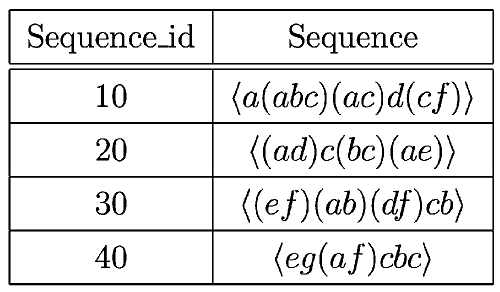
\includegraphics[width=0.35\textwidth]{PrefixSpanOrigDB.png}
    \caption{Original database of our SPM example}
  \end{subfigure}
  \begin{subfigure}{\textwidth}
  	\centering
    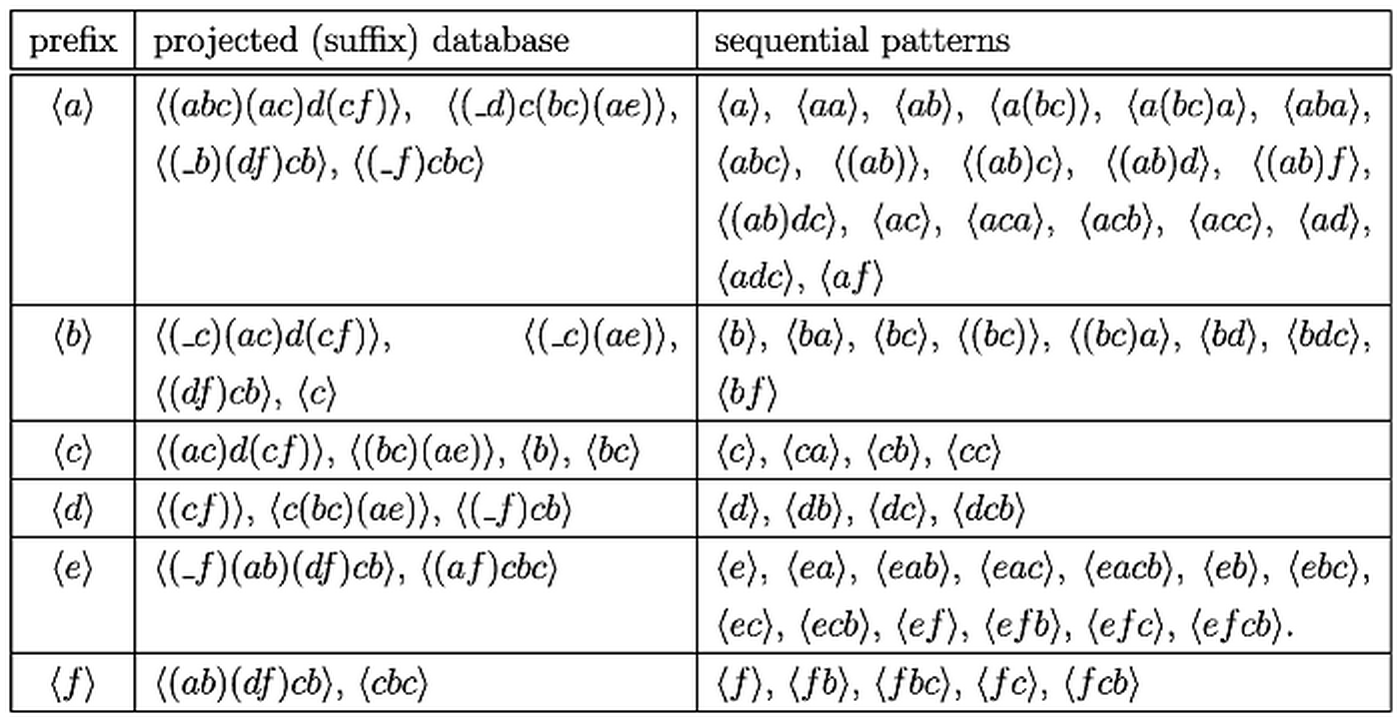
\includegraphics[width=0.9\textwidth]{PrefixSpanProjDB.png}
    \caption[Prefix projected database \& sequential pattern]{
		\tabular[t]{@{}l@{}}
			Prefix projected databases relative to length-1 sequential patterns \& \\
			final list of sequential patterns eventually extended from those length-1 prefixes
		\endtabular
	}
  \end{subfigure}
  \caption{Prefix-Span example}
  \label{ex:PrefixSpanExample}
\end{figure}

The main selling point of the algorithm lies in it's ability to quickly generate candidate extensions, projecting prefixes on the database significantly reducing the time needed to find prefixes extensions, as only the suffixes need to be searched for those extensions to be found. Another selling point lies in it's scalability, as this method is easily implementable under a Map-Combine-Reduce programming scheme. \newline

However, this method also has disadvantages, mainly in the fact that projecting databases is a time expensive process. Making building those projected databases the efficiency bottle-neck of Prefix-Span. \newline

However, techniques exists to break past this bottle-neck and mitigate it's effects. Techniques among which we should mention the 'Bi-level projection' technique, which consist in creating a triangular matrix (S-matrix [\ref{fig:smatrix}]) registering the number of supports for all length-2 sequences that can be assembled from length-1 prefixes. A quick scan of the S-matrix then allows the detection of all supported length-2 prefixes, prefixes which can then be extended again through applying the same technique on their projected database. Thus allowing a reduction of the number of necessary prefix projection during the algorithm, since only half of them are projected. \newline

A second technique we should mention is the 'Pseudo-Projection' technique which is based on keeping and maintaining a start index for each sequence. This start-index registering the lowest position at which the last projected prefix was supported, thus allowing quicker projection of extending prefixes by avoiding to re-project previous prefix elements.
\subsubsection{cSPADE}

The cSPADE algorithm \cite{zaki2001spade} uses combinatorial properties to divide the original sequence pattern mining problem in smaller sub-problems that can be solved independently using simple id-list join operations. This algorithm is thus parallelizable, furthermore the parallelization has a linear scalability with respect to the size of the inputted database. \newline

cSPADE's first step is to compute all length-1 sequential pattern using a simple database scan. Then, we generate all length-2 sequential pattern and count the number of supporting sequences for each pair of item in a bidimensional matrix. Counting the number of supporting sequence being realised through another database scan by first transforming the original vertical representation of the database into an horizontal representation (see Figure \ref{ex:cspadeDatabaseRepr}).

\begin{figure}[h]
  \centering
  \begin{subfigure}[t]{0.4\textwidth}
  	\centering
  	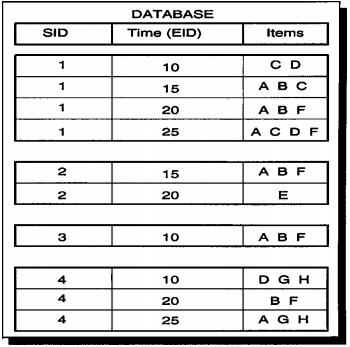
\includegraphics[width=0.95\textwidth]{cspadeVerticalRepr.png}
    \caption{Vertical representation of the database}
  \end{subfigure}
  \begin{subfigure}[t]{0.59\textwidth}
  	\centering
    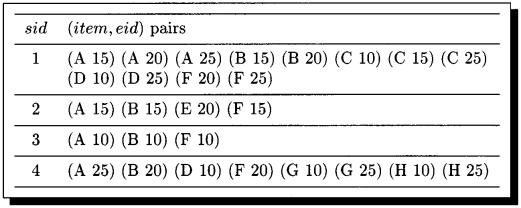
\includegraphics[width=0.95\textwidth]{cspadeHorizontalRepr.png}
    \caption{Horizontal representation of the database}
  \end{subfigure}
  \caption{cSPADE database representation}
  \label{ex:cspadeDatabaseRepr}
\end{figure}

Subsequent length-n sequence patterns can then be formed by joining length-(n-1) patterns using their id-lists (list of positions in sequences for each item, see Figure \ref{fig:cspadeIDList}). The support of each item can also be easily calculated from ID-list, as we just need to count the number of different sequences in which it appears.  \newline

It is also important to note that this method of joining ID-lists is only efficient from length-3 patterns onward, as ID-lists for length 1 and 2 patterns can be extremely large and potentially wouldn't fit in memory. \newline

Of course, at the end of each round, un-frequent sequential pattern should be cleaned as to guarantee only frequent pattern will be extended. This algorithm can be executed using either breadth first or depth first search, and ends it's execution once no patterns can be further extended.

\begin{figure}[h]
  \centering
  \begin{subfigure}[t]{0.54\textwidth}
  	\centering
  	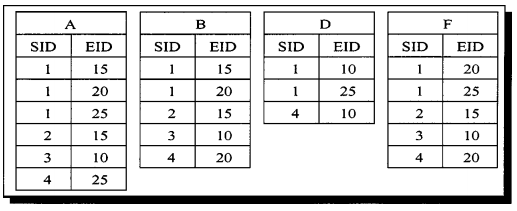
\includegraphics[width=\textwidth]{cspadeVerticalIDList1.png}
    \caption{ID-list of length-1 sequence patterns}
  \end{subfigure}
  \begin{subfigure}[t]{0.45\textwidth}
  	\centering
    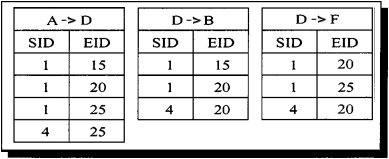
\includegraphics[width=\textwidth]{cspadeVerticalIDList2.png}
    \caption{ID-list of length-2 sequence patterns}
  \end{subfigure}
  \caption{cSPADE's ID-lists}
  \label{fig:cspadeIDList}
\end{figure}

\subsection{Existing CP Based approaches}
\subsubsection{CPSM}

The CPSM approach \cite{negrevergne2015constraint} was implemented to solve sequential pattern mining problems involving only sequences of symbols (no symbols set) using generic Constraint Programming (CP) solvers. It creates a global constraint allowing a search for frequent pattern over the database. Thanks to it's integration in CP solvers, it also easily support additional constraints such as size constraint or regular-expressions constraints. \newline

The global constraint, which form of the basis of this approach, is called the global exists-embedding constraint. Based on an incremental propagator (DFS), the algorithm will incrementally extend a prefix, until no extensions can be successfully projected. \newline

At each step, the solver will take care of assigning the next extensions in our search space. The constraint will then search said extensions to verify it's validity. Of course, the whole sequence won't be searched, but only positions larger than the smallest position supporting the previous valid prefix in each sequence. \newline

If the extension is valid and it's support exceeds the threshold $\theta$, the prefix will be considered 'embedded' in the database. The algorithm thus works by creating all prefixes through various incremental extensions and numerous backtracking, then verifying their embedding in the database. \newline

Since trying all possible extensions at each incremental step would be inefficient, the algorithm was also designed to prune the next possible extensions that should be considered by the solver, and only keep extensions that are sufficiently supported in the database. Thus, symbol that are considered unfrequent won't be branched over during the execution. This pruning is done by counting the number of support for each extensions during the embedding existence verification. \newline

Although impressive for it's modularity, the efficiency of this algorithm didn't quite caught up to specialised non-CP algorithm such as Prefix-Span or cSPADE. It however surpassed their efficiency at searching for specific solution thanks to it's modularity.

\subsubsection{PP}

This second approach based on CPSM proposed a slightly different global constraint by taking idea from prefix-projection \cite{kemmar2015prefix}. Similarly to it's predecessor, this algorithm was designed to solve sequential pattern mining problems involving sequence of symbols (no sets of symbols).\newline

The main idea behind this improved constraint being that we have no need to check sequences for extensions support when they did not support sub-sequences of the current prefix. \newline

This new algorithm thus takes notes of the ID of sequences which support the current pattern so that it's extensions may be projected only on those sequences. The key element of this new feature being that we keep ID of sequence and not copy of sequences, making it extremely memory and time efficient. \newline

During the extensions pruning phase, only supportive sequences will need be checked in a similar fashion, as they are the only relevant sequences to find extensions with. \newline

While the rest of this global constraint implementation was very similar to CPSM, the prefix projection improvement allowed this new implementation to largely overtake it's predecessor in efficiency. Making this new algorithm competitive with state-of-the-art non-CP method while keeping the improved modularity inherent to CP algorithm.

\subsubsection{Gap-Seq}

This new algorithm introduced a global constraint adding support for time gap constraint. This allow, for example, to analyses purchase behaviors and find products usually bought by customers at regular time intervals. \newline

Similarly to it's predecessor, the algorithm was designed to solve sequential patterns mining problems involving sequences of symbols, doing so by incrementally extending and verifying prefixes over multiple pass of a prefix projected database. \newline

The new global constraint however allow tighter search spaces where one can specify the minimal/maximal distance allowed between two symbols for them to remain solution. \newline

For this constraint to work efficiently, additional pruning was added when pruning for extending items, so that extensions which would violate the time gap constraints couldn't be taken into account.

\subsubsection{PPIC}

Largely based on it's predecessor, CPSM and PP, PPIC is an algorithm designed for solving sequence pattern mining problems involving sequences of symbols. Unlike Gap-seq, constraint over time gaps are not supported. \newline

This new algorithm speciality laying in it's record breaking efficiency, surpassing even state-of-the-art non-CP solver, generally by a wide margin (see Figure \ref{fig:PPICvsOther}).

PPIC's implementation is based on the Prefix-Span approach, it's execution can be separated in two stages :

\begin{enumerate}
\item \textbf{Pre-processing :} In this first stage, we first clean the received sequences from unfrequent symbols, renaming them into unique items. Three matrices are then build from the sequence database :
	\begin{enumerate}
		\item The 'first-position' matrix : A \#SDB*N sized matrix allowing O(1) jumps to the first occurrence of a given item. 
		\item The 'last-position' matrix : A  \#SDB*N sized matrix allowing O(1) check for the presence of a given item in the remains of a sequence.
		\item The 'interesting-position' matrix : A matrix with the same size as the original sequence database, but whose content are changed from the items forming those sequences, to the positions of the next 'interesting' item. That is the next position where an item last appears in a sequence. \\ Although, at first glance, this matrix may seem redundant with the last-position matrix, its purpose appears when one realise that to achieve the same goal a whole columns of the last-position matrix would have to be checked. Similarly, keeping only this matrix would also be less efficient, since there would be no way to efficiently check if an item is present in the remains of a sequence. Both matrices are thus needed to achieve the greatest efficiency gain. 
	\end{enumerate}
	
	The pre-processing stage will also take care of adding multiple constraint, depending on the wishes of the user. Thus restricting the search space to fit tightly the desired solutions and improving performances at reaching those specific solutions.
	
\item \textbf{Execution :} Once the pre-processing is finished, the algorithm will truly start to run. Using the three matrices, prefixes will be extended efficiently using an incremental propagator (DFS approach). An approach possible thanks to trailing, that is more efficient than BFS approach were multiple copies of the database would need to be kept, or where the prefixes would need to be re-projected. Thanks to this incremental propagation, memory consumption will thus be minimal during the execution of the algorithm. \newline

Through each step of the DFS execution, the last item of the current prefix will be projected efficiently as, similarly to CPSM, the algorithm keeps track of the minimal index after which the previous valid pattern was considered supported. Thus, only the remains of the sequence will need to be searched for confirming the validity of the new projection. Once projected, the algorithm will then prune possible solutions for the next pattern efficiently, thanks to the lastPosition list, and continue the execution. 

Additionally, to keep the increased performances of the PP algorithm, the algorithm keep notes of which sequences supports the current prefixe while projecting the current extension. For further extensions of the prefix, only those sequences will thus have to be considered during any projection or pruning. Since the algorithm also keep track of the number of support for each extensions, an improvement was also made to stop searching for projections once that number of supporting sequences have been found during the prefix's projection. Since the remaining sequences definitely won't support the item and will remain irrelevant further down this branch of the search tree. \newline

Each time a valid solution is found. That is, a solution that satisfy all constraints injected in the solver. The execution will be momentarily interrupted. The solution will then be translated back to the symbols corresponding to the recorded items and saved in a result list. \newline

Once the solver determines that no further solution can be found under the specified constraints. The execution will terminate, and all resulting pattern will be returned.
\end{enumerate}

An example of a complete execution of PPIC can be found in figure \ref{fig:ppic_exec_example}. The pseudo-code can be found in Algorithm [\ref{alg:PPIC1}, \ref{alg:PPIC2}]. \newline

\begin{figure}[!h]
%\hspace*{-1cm}
\centering
\scalebox{0.5}{
\begin{forest}
for tree={
  draw,
  minimum height=2cm,
  anchor=north,
  align=center,
  child anchor=north
},
[{Input sequences : \\ <ADBABCA> \\ <ABCA> \\ <AD> \\ Number of supporting sequences necessary : 2}, align=center, name=SS
  [{Pre-processed sequences : \\ <1421231> \\ <1231> \\ <14> \\ indexInSequence : \\ $[0, 0, 0]$ \\ supportCounter : \\ $[3, 2, 2, 2]$ \\ firstPosList: \\ $[1, 3, 6, 2]$ \\ $[1, 2, 3, 0]$ \\ $[1, 0, 0, 2]$ \\ lastPosList: \\ $[7, 5, 6, 2]$ \\ $[4, 2, 3, 0]$ \\ $[1, 0, 0, 2]$ \\ interestingPosList: \\ $[2, 5, 5, 5, 6, 7, 0]$ \\ $[2, 3, 4, 0]$ \\ $[2, 0]$}, name=PDC
  		[{Projecting 4 : \\ indexInSequence : \\ $[2, 4, 2]$ \\ sequenceSupported : \\ $[1, 3]$ \\ itemSupportCounter : \\ $[1, 1, 1, 0]$ \\ Extensions supported : \\ \textrm{[]}}
  		]
  		[{Projecting 1 : \\ indexInSequence : \\ $[1, 1, 1]$ \\ sequenceSupported : \\ $[1, 2, 3]$ \\ itemSupportCounter : \\ $[2, 2, 2, 2]$ \\ Extensions supported : \\ \textrm{[1, 2, 3, 4]}}
  			[{Projecting 14 : \\ indexInSequence : \\ $[2, 4, 2]$ \\ sequenceSupported : \\ $[1, 3]$ \\ itemSupportCounter : \\ $[1, 1, 1, 0]$ \\ Extensions supported : \\ \textrm{[]}}
  			]
  			[{Projecting 11 : \\ indexInSequence : \\ $[7, 4, 2]$ \\ sequenceSupported : \\ $[1, 2]$ \\ itemSupportCounter : \\ $[0, 0, 0, 0]$ \\ Extensions supported : \\ \textrm{[]}}
  			]
  			[{Projecting 13 : \\ indexInSequence : \\ $[6, 3, 2]$ \\ sequenceSupported : \\ $[1, 2]$ \\ itemSupportCounter : \\ $[2, 0, 0, 0]$ \\ Extensions supported : \\ \textrm{[1]}}
  				[{Projecting 131 : \\ indexInSequence : \\ $[7, 4, 2]$ \\ sequenceSupported : \\ $[1, 2]$ \\ itemSupportCounter : \\ $[0, 0, 0, 0]$ \\ Extensions supported : \\ \textrm{[]}}
  				]
  			]
  			[{Projecting 12 : \\ indexInSequence : \\ $[3, 2, 2]$ \\ sequenceSupported : \\ $[1, 2]$ \\ itemSupportCounter : \\ $[2, 1, 2, 0]$ \\ Extensions supported : \\ \textrm{[1, 3]}}
  				[{Projecting 121 : \\ indexInSequence : \\ $[4, 4, 2]$ \\ sequenceSupported : \\ $[1, 2]$ \\ itemSupportCounter : \\ $[1, 1, 1, 0]$ \\ Extensions supported : \\ \textrm{[]}}
  				]
  				[{Projecting 123 : \\ indexInSequence : \\ $[6, 3, 2]$ \\ sequenceSupported : \\ $[1, 2]$ \\ itemSupportCounter : \\ $[2, 0, 0, 0]$ \\ Extensions supported : \\ \textrm{[1]}}
  					[{Projecting 1231 : \\ indexInSequence : \\ $[7, 4, 2]$ \\ sequenceSupported : \\ $[1, 2]$ \\ itemSupportCounter : \\ $[0, 0, 0, 0]$ \\ Extensions supported : \\ \textrm{[]}}
  					]
  				]
  			]
  		]
  		[{Projecting 2 : \\ indexInSequence : \\ $[3, 2, 2]$ \\ sequenceSupported : \\ $[1, 2]$ \\ itemSupportCounter : \\ $[2, 1, 2, 0]$ \\ Extensions supported : \\ \textrm{[1, 3]}}
  			[{Projecting 21 : \\ indexInSequence : \\ $[4, 4, 2]$ \\ sequenceSupported : \\ $[1, 2]$ \\ itemSupportCounter : \\ $[1, 1, 1, 0]$ \\ Extensions supported : \\ \textrm{[]}}
  			]
  			[{Projecting 23 : \\ indexInSequence : \\ $[6, 3, 2]$ \\ sequenceSupported : \\ $[1, 2]$ \\ itemSupportCounter : \\ $[2, 0, 0, 0]$ \\ Extensions supported : \\ \textrm{[1]}}
  				[{Projecting 231 : \\ indexInSequence : \\ $[7, 4, 2]$ \\ sequenceSupported : \\ $[1, 2]$ \\ itemSupportCounter : \\ $[0, 0, 0, 0]$ \\ Extensions supported : \\ \textrm{[]}}
  				]
  			]
  		]
  		[{Projecting 3 : \\ indexInSequence : \\ $[6, 3, 2]$ \\ sequenceSupported : \\ $[1, 2]$ \\ itemSupportCounter : \\ $[2, 0, 0, 0]$ \\ Extensions supported : \\ \textrm{[1]}}
  			[{Projecting 31 : \\ indexInSequence : \\ $[7, 4, 2]$ \\ sequenceSupported : \\ $[1, 2]$ \\ itemSupportCounter : \\ $[0, 0, 0, 0]$ \\ Extensions supported : \\ \textrm{[]}}
  			]
  		]
  	  ]
  	]
  ]
]
%\node[anchor=west,align=left]  at ([xshift=-2cm]MS.west) {Level 3\\Criteria};
\end{forest}}
\caption[An example of PPIC's execution]{
	\tabular[t]{@{}l@{}}
		A simple execution of PPIC's algorithm.\\
		The solutions patterns are the projected prefixes
	\endtabular
}
\label{fig:ppic_exec_example}
\end{figure}

\subsection{Parallelisation}
\subsubsection{The Benefits of Parallelisation}
\subsubsection{Tool selection}

Since, fortunately, SPM problems are embarrassingly parallel problem, we had the opportunity to choose from a selection of widely used open-source libraries. We, however, restricted ourselves to Scala compatible framework, as the CP library supporting PPIC was implemented in this language. Rapidly, we were left to choose from two major options :

\begin{enumerate}
\item Hadoop mapreduce
\item Spark
\end{enumerate}

\paragraph{Hadoop}

Hadoop is an open-source framework that allows large-scale data processing across clusters of machine. Based on a Map-reduce programming model, this framework allows larger scale iterative computation on humongous quantities of data. At each iteration, the data is read from the distributed file systm (HDFS), modified through a MapReduce, then stored back on the file system. \newline

The advantages of Hadoop thus lies in the simplicity of it's usage. Aside from implementing the implementing the Map and Reduce process, Hadoop will takes care of scheduling, data repartition and failure recovery. \newline

Widely used since it's Initial release in December 10, 2011. Hadoop slowly climbed to become of the big standards in terms of large scale computation. We thus selected it as our potential scalable framework, discovering shortly after, that an efficient implementation of Prefix-Span on Hadoop was already available on the internet.

\paragraph{Spark}

Spark is an open-source engine for large-scale data processing. Mainly reputed for it's speed, ease of use, and ability to efficiently implement sophisticated problems. \newline

Originally developed at UC Berkeley in 2009, It's entire implementation revolves around an immutable read-only data structure called the \textbf{resilient distributed dataset (RDD)}. Maintained in a fault-tolerant way, those lazily computed RDD, built through deterministic coarse-grained transformation, have been designed to be efficiently distributed over a cluster of machines, allowing resolution of complex iterative problem in scalable environments. \newline

Furthermore, Spark's has been designed to make use of it's clusters RAM memory efficiently, allowing the engine distance itself from slow HDD memory access. Of course, should the RAM memory be insufficient, Spark is perfectly able to run using nothing but the hard-drive. \newline

Spark's was thus an extremely valid choice from a technical standpoint and, similarly to Hadoop, we were surprised to discover an existing implementation of Prefix-span available in Spark's machine learning library.

\paragraph{Final choice}

As said earlier, both of those libraries already disposing of a scalable PrefixSpan implementation. It was thus a matter of determining whose performances were better, and whether those implementations could be efficiently extended through CP technologies. \newline

Fortunately for us, performance comparison had already been done in a widely recognised scientific paper on Spark's RDD \cite{RDD}. Those performances are presented in Figure \ref{fig:hadoopVSspark}

\begin{figure}[h]
  \centering
  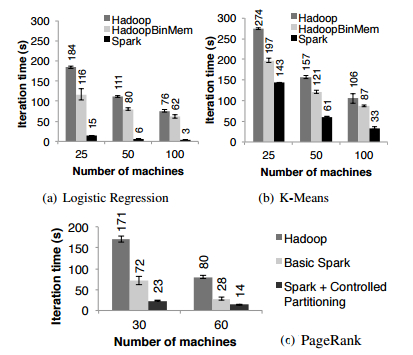
\includegraphics[width=0.6\textwidth]{hadoopVSspark.png}
  \caption{Performance comparison of Hadoop and Spark}
  \label{fig:hadoopVSspark}
\end{figure}

As you can see, performance-wise, Spark vastly outperform Hadoop thanks to its ability to use both memory and disk for it's computations. Allowing up to 100x speed-up under the right circumstances, as you can see in the logistic regression problem. According to the official website, Spark would also boast a 10x speed-up through on disk computation, but no performance benchmarks were provided. \newline

In terms of extensions through CP technologies, we quickly realised that Hadoop would be far less practical. Although MapReduce can be used to execute the standard PrefixSpan algorithm, and could certainly be modified to introduce CP elements, Spark can support any coarse-grained transformation with its RDDs, allowing a more precise implementations where only required transformations would be made, instead of simple sequences of Map-Combine-Reduce. \newline

\section{Implementation of a Scalable CP Based Algorithm}

In this section, we shall present the various implementation we created in an attempt to improve Spark's original algorithm's performances. Be it through the addition of CP based algorithms and techniques, or more directly. \newline

The performance of those algorithm will however be tested in a later section.

\subsection{Spark's original implementation}

Before introducing our various implementation, let us present the original algorithm.
Spark's algorithm is based on the Prefix-Span approach, and can be separated in four stages :

\begin{enumerate}
\item \textbf{Pre-processing :} The goal of this stage is to replace each item of the sequence database by an unique ID, to separate itemSets by a zero delimiter, and to clean the database from unfrequent items. \\
For example, the sequence <(ABD)(ABC)A> will become 0120123010, assuming only items A, B and C are frequent in the sequence database.
\item \textbf{Scalable execution :} The core of the algorithm. Its execution consist in extending prefixes through a three sub-stage process, starting from the empty prefix.
	\begin{enumerate}
	\item First, a large prefix is projected on the database. If there is no prefix to project, the scalable execution comes to an end and the solutions will be returned.
	\item Then, from the set of supporting sequences, we discover symbols that can extend the current prefix. If no such extension exists, we try the next large prefix.
	\item Finally, for each possible symbol extension, we extend the prefix. we then determine how long further expanding each extended prefix may take by calculating the projected database size. Depending on the calculated projected size and of the value of a user defined parameter, we then either further extend this prefix using another iteration of scalable execution, or store it for use in the local execution stage. 
	\end{enumerate}
\item \textbf{Local execution :} The local execution is completely similar in its implementation to the scalable execution. Its only use is in improving the algorithm's performance by calculating all extensions from a Prefix locally, instead of doing so while shuffling information around the scalable architecture. \\
This stage is only launched once all large prefixes have been extended sufficiently, making the databases needed for future extensions small enough. Depending on the parameters inputted by the user, this stage may be skipped. TODO: add performance difference of keeping database on shuffle file.
\item \textbf{Post-processing :} During the post-processing step, we translate back the unique IDs into the item they each represented. Then we send back the collected results to the user.
\end{enumerate}

During the prefix projection phase of the scalable and local execution, the algorithm will also detect which item-sets in the sequence comply with what has already been projected and can still be extended in some way. Storing such items positions in a 'partial projection' list. \newline
That way, if we are projecting an item-set containing multiple symbol from a prefix, until the end of that item-set, the items projection phases will know where to search possible extensions, preventing the algorithm from having to search the whole sequence. \newline
Also, should we be computing a single-item pattern mining problem, no partial start would be created and kept in memory, since the algorithm automatically detect that those item-sets cannot be extended. \newline

If the item-set end, the full remains of the sequence, from the earliest partial position recorded, will have to be searched. During this search, new potential partial projection will be recorded, and the old ones will be discarded. \newline

During the prefix extension phase, the current partial projection will also be used to find extensions of the current itemset quicker. The remainder of the database will also be searched, but only for extension that starts new itemsets. \newline

An example of a fully scalable execution from this algorithm can be found in figure \ref{fig:spark_exec_example}. A pseudo can also be found in Algorithm [\ref{alg:SPARK1}, \ref{alg:SPARK2}, \ref{alg:SPARK3}]. \newline

\begin{figure}[h]
\centering
\scalebox{0.55}{
\begin{forest}
for tree={
  draw,
  minimum height=2cm,
  anchor=north,
  align=center,
  child anchor=north
},
[{Input sequences : \\ <(ADB)(ABC)(A)> \\ <(ABC)A> \\ Number of supporting sequences necessary : 2}, align=center, name=SS
  [{Pre-processed sequences : \\ <0120123010> \\ <0123010>}, name=PDC
  	[{Empty prefix projection : \\ <|0120123010> \\ <|0123010> \\ Partial starts : \\  \textrm{[]} \\ \textrm{[]} \\ Extensions found : \\ \textrm{[01, 02, 03]}},
  		[{Projecting 01 : \\ <01|20123010> \\ <01|23010> \\ Partial starts : \\  \textrm{[4]} \\ \textrm{[]} \\ Extensions supported : \\ \textrm{[2, 3, 01]}},
  			[{Projecting 0101 : \\ <012012301|0> \\ <012301|0> \\ Partial starts : \\  \textrm{[]} \\ \textrm{[]} \\ Extensions supported : \\ \textrm{[]}}]
  			[{Projecting 013 : \\ <0120123|010> \\ <0123|010> \\ Partial starts : \\  \textrm{[]} \\ \textrm{[]} \\ Extensions supported : \\ \textrm{[01]}},
  				[{Projecting 01301 : \\ <012012301|0> \\ <012301|0> \\ Partial starts : \\  \textrm{[]} \\ \textrm{[]} \\ Extensions supported : \\ \textrm{[]}}]
  			]
  			[{Projecting 012 : \\ <012|0123010> \\ <012|3010> \\ Partial starts : \\  \textrm{[5]} \\ \textrm{[]} \\ Extensions supported : \\ \textrm{[3, 01]}},
  				[{Projecting 0123 : \\ <0120123|010> \\ <0123|010> \\ Partial starts : \\  \textrm{[]} \\ \textrm{[]} \\ Extensions supported : \\ \textrm{[]}},
  					[{Projecting 012301 : \\ <012012301|0> \\ <012301|0> \\ Partial starts : \\  \textrm{[]} \\ \textrm{[]} \\ Extensions supported : \\ \textrm{[]}}]
  				]
  				[{Projecting 01201 : \\ <012012301|0> \\ <012301|0> \\ Partial starts : \\  \textrm{[]} \\ \textrm{[]} \\ Extensions supported : \\ \textrm{[]}}]
  			]
  		]
  		[{Projecting 03 : \\ <0120123|010> \\ <0123|010> \\ Partial starts : \\  \textrm{[]} \\ \textrm{[]} \\ Extensions supported : \\ \textrm{[01]}},
  			[{Projecting 0301 : \\ <012012301|0> \\ <012301|0> \\ Partial starts : \\  \textrm{[]} \\ \textrm{[]} \\ Extensions supported : \\ \textrm{[]}}]
  		]
  		[{Projecting 02 : \\ <012|0123010> \\ <012|3010> \\ Partial starts : \\  \textrm{[5]} \\ \textrm{[]} \\ Extensions supported : \\ \textrm{[3, 01]}},
  			[{Projecting 0201 : \\ <012012301|0> \\ <012301|0> \\ Partial starts : \\  \textrm{[]} \\ \textrm{[]} \\ Extensions supported : \\ \textrm{[]}}]
  			[{Projecting 023 : \\ <0120123|010> \\ <0123|010> \\ Partial starts : \\  \textrm{[]} \\ \textrm{[]} \\ Extensions supported : \\ \textrm{[01]}},
  				[{Projecting 02301 : \\ <012012301|0> \\ <012301|0> \\ Partial starts : \\  \textrm{[]} \\ \textrm{[]} \\ Extensions supported : \\ \textrm{[]}}]
  			]
  		]
  	]
  ]
]
%\node[anchor=west,align=left]  at ([xshift=-2cm]MS.west) {Level 3\\Criteria};
\end{forest}}
\caption[An example of Spark's execution]{
	\tabular[t]{@{}l@{}}
		A simple execution of Spark's algorithm.\\
		The solutions are the projected prefixes (except the empty prefix)
	\endtabular
}
\label{fig:spark_exec_example}
\end{figure}

\begin{itemize}
  \item[NB:] During our first analysis of Spark's pre-processing stage, we noticed a small inefficiency in the cleaning of the database's sequences. When multiple itemsets were fully cleaned of their item, the algorithm had a tendency of creating sequences of zero delimiters, as the algorithm still delimited empty itemsets.

Although the internal representation was still correct and results weren't modified, those trailing zeroes substantially slowed the algorithm down.
The performance improvement of this small correction is reflected in the annexes, figure \ref{spark_preprocessing_fix}.

Later, this small correction was proposed to Spark's community and quickly accepted into the default implementation. In the remains of this paper, we will thus consider this corrected version which has been approved by the community as the original algorithm for Spark, and compare our performance improvement with this corrected version as the basis.
\end{itemize}

\subsection{A First Scalable CP based Implementation}

As mentioned earlier in this paper, Spark's original algorithm is composed of two different execution stages. We thus analysed each stage independently to understand how CP technique could improve their implementation. Although we rapidly discovered that the scalable stage could hardly be modified to efficiently incorporate CP techniques, at least not without completely incorporating Spark into the solver, we realised that the local execution stage could be significantly improved. \newline

In fact, the entire local execution could be easily replaced by a CP based algorithm. For \acrshort{SoS} problems where PPIC is applicable, we could even use a nearly identical implementation where only the pre-processing would need to be modified as to fit Spark's middle-put. \newline

To remain able to solve \acrshort{SoSS} problems through a local execution. A simple boolean was also added, so that user could specify whether PPIC could be used on the input dataset. \newline

This implementation's pseudo-code can be found below, in Algorithm \ref{alg:FirstImplem}.

\subsection{Improvements Pathways}

To improve this first scalable CP based implementation, we identified three promising options that needed to be studied:

\begin{enumerate}
	\item Improve the link between Spark's middle-put and PPIC's input. The easiest option, but also the most promising, since both algorithm have been separately optimised in terms of performances.
	\item Improve Spark's performances by incorporating more idea's from pattern mining.
Which would improve both the scalable execution and the original local execution component of Spark. Thus improving performances on both single and multi-item pattern problems.
	\item Developing a new version of PPIC which can efficiently be applied to multi-item pattern. Making CP usable for every local execution opportunity and, hopefully, improving performances.
\end{enumerate}

Additionally to those performance improving options, we also decided to prove that PPIC's modularity can be conserved in a scalable environment through the addition of multiple  functionalities in our future implementations.

\subsection{Adding new functionalities}

To first task we undertook was to add four new functionalities to our first CP based Implementation. The implemented functionalities were as follow :

\begin{enumerate}
	\item Unbounded max pattern length : Although Spark's implementation already disposed of a way to control the maximum length of a pattern, no special value existed to allow unlimited max pattern length. We thus added this minor functionality, specifying 0 as a special value that would allow searching for all solutions pattern of any length. Additionally, we changed the default value of 10 to this new special value, so that all solutions could be found by default.
	\item Min pattern length : Although Spark's original implementation allowed to control the maximal length of a pattern. No such functionalities existed to control their minimal length. We thus added a functionality to specify the minimal length a pattern should have before being considered solution. As all pattern containing less non-zero item that the specified input wouldn't be in-putted, we decided to set the default value of this parameter at 1, so that solution wouldn't be restricted.
	\item Limit on the maximal number of item per item-set : This functionality was added so that user could, once again, better control their outputted results. Supposing an hypothetical business would like to find all sequences of item bought in pair in a dataset, it would have no need for solutions where item-sets are larger than two. We can thus stop searching for further item-set extensions once the limit has been reached and, de-facto, improve our algorithm performances for returning those specific solutions. Additionally, we created a special value (0) so that all item-set of any length could be outputted, and set that special value as our default for this parameter.
	\item Soft limit on the number of sub-problems created : By default inactivated, this parameters is enabling far better performance on protein like datasets where projected databases tend to have rather similar sub-problems. Its implementation is a simple check at the beginning of each iteration of the scalable algorithm. If the number of sub-problem created is larger than the user inputted value, the implementation will forcefully put an end to the scalable stage, and switch to a local execution on each worker.
	For the default value of this parameter, a special value (0) was created so that the number of created sub-problems wouldn't be limited.\newline
	
	 As you can see in Figure \ref{fig:sub_problem_limit}, performance improvement are only observed on the protein, Kosarak, slen2 and slen3 datasets, but the increase in performance is significant. The problem being that the loss of performance on other datasets is generally even more significant. This loss in performance comes from large differences in sub-problems sizes appearing due to the forced local execution. Since the largest problems tend to be created and processed last, only a few executor have problems to work on toward the end of the execution. The remaining executor staying idle for the reminder of the local execution stage. Moreover, those remaining problems take a very long time to compute, greatly slowing down the measured performance. \\
	 As is, this parameter should be used with extreme care. However, we will consecrate a section to studying possible improvement of its performances later in this paper. TODO : add link to that section.
\end{enumerate}

While these additions did not have any measurable impact on performances at their default value, they still allowed better control of the search space. Proving that, although using a CP solver in Spark seriously affected modularity, a certain level could be easily kept from the original CP solver. \newline

A pseudo-code demonstrating the changes brought to the code can be found in Algorithm \ref{alg:NF}.

We then looked into improving our performances, leading the the discovery of two potential inefficiencies.

\subsubsection{Quicker - Start}

During the pre-processing of Spark's original implementation, unfrequent items are cleaned from the database. Frequent items are thus found in the process, only to be discarded and searched for once more when projecting an empty prefix at the beginning of the scalable execution. \newline

We thus modified our first CP implementation to remove this 'inefficiency', deciding to pass frequent-item directly to the scalable stage, instead of discarding them before searching for them once more through a complete iteration over the database. \newline

The code was modified accordingly, as shown in Algorithm \ref{alg:QuickStart}.

\subsubsection{Cleaning Sequence before the Local Execution}

The next inefficiency we found was that, during PPIC's local execution, three matrices were build whose size depended on the number of  unique symbols in the input databases.
Yet, in our first implementation, the various projected Databases that reached the local execution stage often had unfrequent symbols that could potentially be cleaned. \newline

Cleaning them would not only reduce the input database's size, it would also reduce the size of those matrices. Making it a potentially worthwhile deal to pre-process PPIC's input for each projected databases of the local execution. \newline

We thus modified our code accordingly, producing a code similar to Algorithm \ref{alg:CleanBeforeLocalPPIC} \newline

Since, as we will see later in the performance testing section, large increase in performances can be observed through these two improvements, and since so many other improvements needed to be implemented, \textbf{we decided to use this implementation as reference for the remainder of this paper}. All further improvement were thus added separately to this version, later allowing us to better compare the performance gains brought by each implementation. \newline

We will thus end this implementation section with a final implementation regrouping all implementation which showed performance improvements.

\subsection{Improving the Switch to a CP Local Execution}

In this section, we will discuss the improvement we tried to bring to the translation from Spark's middle-put to our local executions input, and the results we obtained. For each improvement, we will explain its nature and the trade-off's its implementation may encompass.

\subsubsection{Automatic Choice of the Local Execution Algorithm}

Our next attempted improvement was to automatise to choice between PPIC and Spark's local execution. Using the former only for \acrlong{SoS} problems, and the latter for \acrlong{SoSS} problems. \newline

This would allow to be more efficient by default, without needing involvement from the user to decide whether PPIC or Spark's original local execution should be used.

In that endeavour, we decided to recalculate the maxItemPetItemSet argument dynamically during the pre-processing stage. Since it allow us to determine whether we were dealing with \acrshort{SoS} or \acrshort{SoSS}, and thus, whether PPIC could be used during the local execution. \newline

Additionally, should maxItemPerItemSet be left to it's default value or should it have been put to a much too high value, we could theoretically slightly improve performance by refraining from searching extensions to solution pattern having already reached the max recalculated length. Of course, this theoretical performance gain would only apply for databases where the number of Items per item-set do not vary too much.\newline

But this additional feature would be worth a small loss on \acrshort{SoSS}, as long as the usage of PPIC could be guaranteed on \acrshort{SoS}. \newline

Of course, should the non-recalculated parameters be in use, only the requested solutions would be computed.

A pseudo-code demonstrating the implementation of this Automatic choice can be found in Algorithm \ref{alg:AutomaticSelection}

\subsubsection{Generalised Pre-Processing Before the Local Execution}

Extending our previous idea of cleaning the sequence database before PPIC's execution, we decided to create an implementation where the database would be cleaned before any local execution, including \acrshort{SoS} problems. Wondering, if cleaning the sequence database before Spark's original local execution could bring similar improvements. \newline

We thus designed a new cleaning process suited both for Spark and PPIC's local execution input. During this process, we also realised we could also easily check whether the cleaned sequences could be solved using PPIC or Spark. We thus decided to include this feature too, and to compare it's performance gain to our previous maxItemPetItemSet based implementation.

While creating this new implementation, we also discovered more than a few inefficiencies on the old one. Such as the use of ArrayBuffer structure instead of the much more efficient ArrayBuilder, or un-needed extra iteration during the matrices creation. \newline

We thus expected this new implementation to be more efficient on both type of problems and, hopefully, for every dataset.

A pseudo-code representing this implementation can be found in Algorithm \ref{alg:CleanBeforeLocal}.

\subsection{Improving the Scalable Execution}

In this section, we will discuss the improvement we tried to bring to Spark, and the results we obtained. For each improvement, we will first explain its nature and the trade-off's its implementation may encompass.

\subsubsection{Position lists}

The first idea we had to improve Spark's performances, was to use LAPIN's position list to our advantage. \newline

In Spark's original implementation, the scalable and local stages of the algorithm perform their duty in three phases. First they receive a solution prefix which needs to be extended, and project it on the whole database, allowing them to know which sequence support that prefix. Then, in the supporting sequences only, they search for symbols which may extend the prefix. Finally, If some symbols are found and they respect the constraint applied to the solutions, Spark's will save them as solution and try to extend them further. \newline

While this implementation is very efficient in a scalable environment, we thought it could be improved through the addition of position list. More specifically, during the prefix projection phase, we determined it would improve performance if the algorithm knew earlier when a sequence couldn't possibly hold the currently projected pattern, or if the algorithm didn't have to analyse half of the sequence before starting to project this aforementioned pattern. \newline

Of course, the trade-off would be a more import use of memory, as the positions list would need to be kept on RDD along side sequences. To adopt this solution, the improvement would thus need to be important enough to motivate the benefits of the trade-off. \newline

From this idea, we implemented three new implementation. The first using only a last position list, the second using only a first position list, and the last using both position-list together. \newline

In Algorithm \ref{alg:posLists}, you will find a pseudo-code of the implementation including both positions lists together.

\subsubsection{Specialising the Scalable Execution}

To improve the scalable execution's performances further, we then had the idea to separate the scalable execution stage of \acrshort{SoS} and \acrshort{SoSS} problems.

This idea stemming that, for \acrshort{SoS} problems, the database internal representation could be seriously improved by removing unnecessary separator. Effectively reducing the size of their internal representation by two. \newline

We thus implemented a new scalable stage specialised for \acrlong{SoS} problems. It's main features being the absence of spacial start and the much more compact database representation without delimiters. \newline

A trade-off was however made, as we now needed to detect in which type of pattern mining problem we were before starting the execution. We needed to create a different database for each type and simply removing the delimiters after a check wouldn't have been efficient. \newline

The most efficient way we found to detect the type of problem was during the frequent symbol detection part of the pre-processing step. Where we could efficiently detect whether each sequence could be use the shortened representation. \newline

The problem being that sequence which could be solved by a \acrlong{SoS} problems after cleaning would never be detected. However, since this case rarely appear over a whole database, we decided checking before cleaning would be sufficient for our purposes. \newline

We thus put performance forward, implementing the code found in Algorithm \ref{alg:SpecializedScalableExec}.

\subsubsection{Priority Scheduling for Sub-Problems}

The final idea we explored to improve Spark's performance, was to modify the order in which sub-problems are computed during the local execution stage. \newline

In the original code, problem are decomposed until they become smaller than a size specified by the 'maxLocalProjDBSize' parameter. As mentioned before, in our reference algorithm, an extension of that idea, the subProblemLimit parameter, was also implemented to allow better control of the number of created sub-problem. \newline

However, we have seen that a consequence of this new functionality is that sub-problems can largely vary in size, making some problem far harder to solve than others. Something would rarely appear in the original version. Coincidentally, we also realised that major drops in performance were experienced if those large problem were solved last, since some executor would be left with nothing to do while other would be stuck with atomic large workload.
\newline

The solution was clear, large problems needed to be solved first in the various executor, so that smaller workload could be shuffled between executor in the later stage of the execution.

\paragraph{Analysing sub-problem creation}

The piece of code which created the various sub-problems from the various projected prefixes collected during the scalable stage, was fundamentally a mapReduce process. The sequences from the original sequence database being projected one by one with different prefixes, then mapped to some reducer, depending on the prefix's ID 
(see Figure \ref{fig:sparkMapReduce}). \newline

\begin{figure}[h]
  \centering
  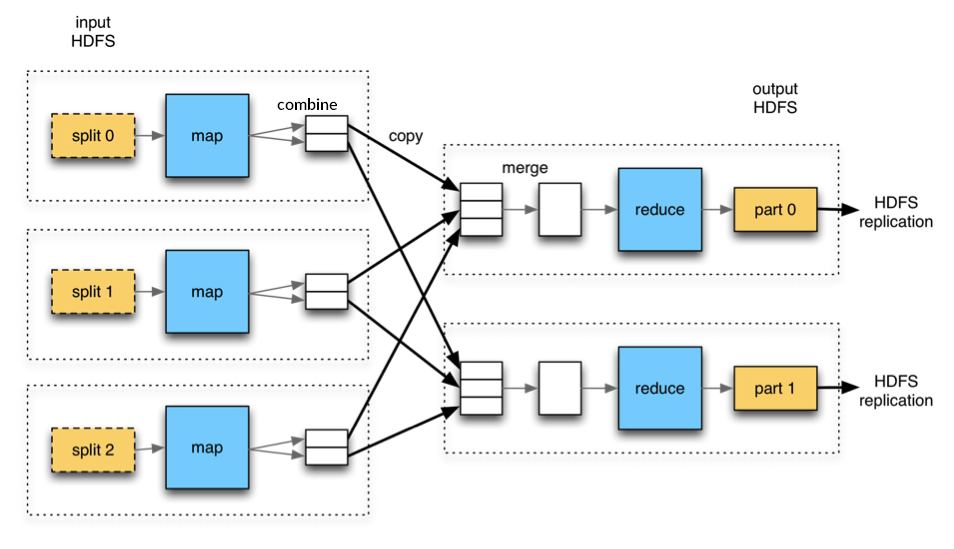
\includegraphics[width=0.8\textwidth]{sparkMapReduce.png}
  \caption{Spark's mapReduce}
  \label{fig:sparkMapReduce}
\end{figure}

\paragraph{Sort sub-problem on the reducer}

We thus concluded a simple solution could be implemented. According to the specification of Spark's sortBy function, the sorting stage will be exacted locally on each reducer. We thus implemented this quick change by adding a simple sort between our map and reduce stage, obtaining the implementation found in Algorithm \ref{alg:sortReducer}.

But, as you will see during our performance tests, although this algorithm produced better performance. A memory issue now appeared, to the point of crashing our 10G executor. \newline

As it turns out, to sort the various sub-problems depending on their size, Spark's obviously needs to evaluate and hold in memory all sub-problems assigned to an executor.
Only then could Spark sort them, all the while while keeping those sub-problems either on disk or memory. \newline

To remain scalable, we thus had to come up with another solution to sort our sub-problems. One that did not involve computing multiple sub-problem and keeping them in memory..

\paragraph{Sort sub-problem on the mapper}

We thus realised we needed to sort our sub-problems during the mapping phase of the mapReduce. After a few trial and error, we realised that the mapping function of Spark created sub-problem one by one, following the mapping code and sent them directly to the reducer through the groupBy function, which delivered them in the very same order they were sent. \newline

We thus modified our implementation to change the order in which we created our sub-problem, instead of sorting them afterwards. The created sub-problems would now be mapped to the reducer and computed in the same order that they were mapped.\newline

Meaning that, by mapping the hardest problems first, they would also be executed first. \newline

We then modified our code to sort our prefixes in descending order through their projected database size, a size which was already computed during the scalable stage of our algorithm, and could simply be stored in the prefix until used to sort. This made sorting sub-problems far more efficient, at a small cost in memory. \newline

As expected, sorting a few prefixes used an insignificant amount of memory in comparison to sorting huge RDD containing complete projected database, while producing equivalent, if not better, performances. As you will see in the dedicated performance testing section. \newline

A pseudo-code based on the implemented changes can be found in Algorithm \ref{alg:sortMapper}

\subsection{CP Based Local Execution for Sequence of Sets of Symbols}

Our final implementation attempts, were to create a CP-based implementation to solve pattern mining problems involving sets of symbols. Of course, to replace the original local execution, this implementation would need to be more performant than it's predecessor.

\subsubsection{Pushing PPIC's Ideas Further}

Our first attempt at creating such an implementation, was to try pushing PPIC's ideas further. \newline

We decided to forgo all three pre-computed matrices, and to change the structure of our sequence database to fill those matrices purposes more efficiently. Instead of an array, we changed each sequence into a map containing unique symbols as key and the various positions of each key symbol as value. \newline

Additionally, we represented the sequence's symbols positions (including zero delimiter position) by a ReversibleArrayStack structure, thus allowing efficient backtracking of the remaining position of a symbol through trailing. \newline

This new structure's purpose was to allow us to make distant jumps and checks more efficiently, at the cost of an higher memory consumption. Theoretically, finding the next position of a given symbol would be O(1), be this next position the last or first position of the symbol. Should the symbol's position list be empty, or should the last recorded position be smaller than our current position in the sequence, we would also immediately know that no more such symbol were contained in the remains of the sequence. \newline

The trade-off lied in the number of reversible point that needed to be maintained. With one ReversibleArrayStack per symbol for each sequence. This number could grow quite quickly, the results may thus greatly vary between datasets but we had good faith it the performance tests would yield satisfying results.

Translating our improvement to pseudo-code, we obtain Algorithm \ref{alg:PPICMAP}.

\subsubsection{Adding Partial Projections to PPIC}

We decided to try another approach at developing an efficient CP based implementation for problems involving sequences of sets of symbols. This second attempt focusing on bringing the partialStart structure of Spark to be used in a PPIC like algorithm. \newline

First we realised that keeping all three matrices wouldn't be efficient. In a set of symbol pattern mining context. To keep the same function, the 'interesting position' matrix needed to be modified to indicate the next last appearance of an item in an itemset, instead of the next last appearance of an item in the sequence, as it did before. This in turn, makes this matrix useless as the next such position would nearly always be the next item of the database. \newline

We thus decided to remove this matrix, but to keep the first and last positions lists, as they remained relevant.
We also modified our implementation to keep zero delimiters during cleaning and to change the partial start received from Spark during the pre-processing, so that they still referred to the same item-set after cleaning (lest the item-set completely disappear in which case that particular partial start will be scraped). \newline

The disadvantage of partial starts however, was that they need to be maintained and advanced at each step of our DFS execution. This meant that, when starting a new item-set, all remaining sequences of the database would need to be fully explored. \newline

For item-set extensions however, only the position list as partial starts would need to be checked, along the sub-sequent position before the next separator, thus we expect greater performance improvement the longer item-sets could extended. \newline

\todo[inline]{TODO : Pseudo code}

\addtocontents{toc}{\protect\newpage}
\section{Performances}

To compare the performances of our various implementations, we first need to discuss how those performance were measured, and on which dataset they were measured.

\subsection{Datasets}

For our performance tests, eight datasets were chosen for the different characteristic they displayed. The goal being to prove the efficiency of the developed algorithm in a wide range of situations. The chosen datasets and their characteristic are displayed in Table \ref{tab:datasets} : \newline

\begin{table}[h]
  \centerline{
  \begin{tabular}{| c | l | c | c | c | c | c | c | r |}
  	\hline
  	& Dataset & \#SDB & N & avg(\#S) & avg(\#Ns) & max(\#S) & Sparsity & description \\
  	\hline
  	\multirow{6}{*}{1.} 
  	& BIBLE & 36369 & 13905 & 21.64 & 17.85 & 100 & 1.18 & text \\
  	\cline{2-9}  
  	& FIFA & 20450 & 2990 & 36.24 & 34.74 & 100 & 1.19 & web click stream\\
  	\cline{2-9}  
  	& Kosarak-70 & 69999 & 21144 & 7.98 & 7.98 & 796 & 1.0 & web click stream\\
  	\cline{2-9}  
  	& LEVIATHAN & 5834 & 9025 & 33.81 & 26.34 & 100 & 1.25 & text\\
  	\cline{2-9}  
  	& PubMed & 17237 & 19931 & 29.56 & 24.82 & 198 & 1.17 & bio-medical text\\
  	\cline{2-9}  
  	& protein & 103120 & 25 & 482.25 & 19.93 & 600 & 24.21 & protein sequences\\
  	\hline
  	\multirow{3}{*}{2.} 
  	& slen1 & 50350 & 41911 & 13.24 & 13.24 & 60 & 1.0 & generated dataset\\
 	\cline{2-9}  
  	& slen2 & 47555 & 62296 & 17.97 & 17.97 & 74 & 1.0 & generated dataset\\
  	\cline{2-9}  
  	& slen3 & 287676 & 81368 & 17.07 & 17.07 & 85 & 1.0 & generated dataset\\
  	\hline
  \end{tabular}}
  \caption[Dataset features]{
  	\tabular[t]{@{}l@{}}
  		Datasets features. The datasets of category 1 contain only \acrshort{SoS}, \\
  		while the datasets of category 2 contain only \acrshort{SoSS} \\
  		- \#SDB = number of sequences; \\
  		- N = Number of different symbols in the dataset; \\
  		- \#S = Length of a sequence S; \\
  		- \#Ns = Number of different symbols in a sequence S; \\
  		- Sparsity = $\frac{1}{\#SDB} * \sum \frac{\#S}{\#Ns}$
  	\endtabular
  }
  \label{tab:datasets}
  %\caption{Datasets features. \#SDB = number of sequences; N = Number of different symbols in the dataset; \#S = Length of a sequence S; \#Ns = Number of different symbol in a sequence S; sparsity = $\frac{1}{\#SDB} * \sum \frac{\#S}{\#Ns}$}
\end{table}

As you can see, our datasets vary largely in their characteristic, be it in their sparsity or in the size of their set of symbols. Although the selected datasets focus slightly more on \acrlong{SoS}, since it has been our focus in most of our developed improvement, we also made sure to correctly represent \acrlong{SoSS} with our last three datasets. \newline

\subsection{Number of Partitions}

As seen previously in Figure \ref{fig:hadoopVSspark}, Spark's performance may vary greatly depending on the number of partitions created from the Input dataset.\newline

The number of created partition must thus be carefully selected as, should there be too much partitions created, the algorithm will lose considerable amount of time switching its execution between partitions. Also, should there be too little partition, scalability may be affected, as executor will need to hold large partitions in memory. In extreme cases, Spark's shuffler may even crash while shuffling partitions around. \newline

We have thus decided to keep a constant, carefully selected, number of partitions for each dataset. So that our performances performance can remain comparable while guaranteeing a complete absence of shuffler crash due to large partitions.\newline

The number of partitions created for each dataset are displayed in Table \ref{tab:numPartitions}. As you can see, the number of created partition is closely related to the database's size.

\begin{table}[h]
  \centering
  \begin{tabular}{| c | c | c |}
  	\hline
  	Dataset & File size (Ko) & Number of partitions \\
  	\hline
  	BIBLE & 3065 & 250 \\
  	\hline
  	FIFA & 2594 &300\\
  	\hline
  	Kosarak-70 & 2166 & 250\\
  	\hline  
  	LEVIATHAN & 713 & 100\\
  	\hline
  	PubMed & 1646 & 200\\
  	\hline
  	protein & 126046 & 5000\\
  	\hline
  	slen1 & 5400 & 500\\
 	\hline 
  	slen2 & 6896 & 500\\
  	\hline
  	slen3 & 39654 & 1000\\
  	\hline
  \end{tabular}
  \caption{Number of partitions used during performance tests}
  \label{tab:numPartitions}
\end{table}

\subsection{Performance Testing Procedure}
\subsubsection{Distribution Choice \& Cluster Architecture}

Our performances will be tested running different custom distribution of Spark, compiled independently for each specific implementation. The goal being to test the performances of an actual distribution containing our changes, rather than simply running the program on an existing distribution. \newline

Although this will take us longer to obtain results, the goal behind this choice, is that our code could then easily be proposed as the standard for future distributions of Spark.  \newline

Additionally to that, unless specified otherwise, our algorithm will be executed on Spark's standalone cluster, in client deploy mode (not locally). More specifically, during our tests, we will run a simple architecture composed single master and a worker with four executor. A representation of this simple architecture is available in Figure \ref{fig:test_architecture}.\newline

Both the driver and the executors will also dispose of a large amount of memory (10G each) during our tests. As it serves no purpose to limit their abilities when purely comparing performances. \newline

Later in our paper, scalability performances will also be tested in larger, memory-restricted, architecture. The architecture then used shall be specified at the beginning of the concerned section.

\begin{figure}[h]
  \centering
  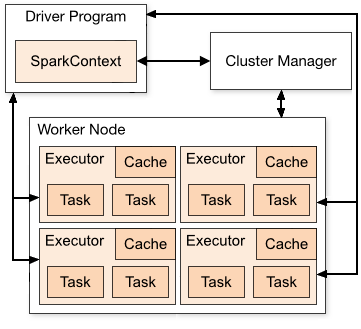
\includegraphics[width=0.45\textwidth]{test_architecture.png}
  \caption{The simple architecture used during the majority of our tests}
  \label{fig:test_architecture}
\end{figure}

\subsubsection{Program Parameters}

At all time, unless specified otherwise, the program parameters will be kept at their default value, so that differences in parameters will never be reflected in our performance comparisons.\newline

An exception to that rule being the 'maxPatternLength' parameter of Spark, which its default value of 10 doesn't fit our purpose as it prevent all sequences to be found on our largest datasets. We will thus use INTEGER.maxValue instead, so that every solution pattern from our datasets may be outputted.\newline

Also, as mentioned previously, all additional functionalities implemented have been designed to affect performance as little as possible when left to their default value. Their default value will thus similarly be used, unless specified otherwise before the performance test.

\begin{itemize}
  \item[NB:] As you will see further down in our performances tests, a section has been dedicated to comparing the performance of our final algorithm under default and optimal parameters. As you will see, performance improvement can be quite substantial. \todo[inline]{TODO : Prove it}
\end{itemize}

\subsubsection{Measurement Span}

For our performance tests, we will measure not only the running time of our algorithm, but also its pre-processing and dataset loading performances. The aim being to develop a new implementation that entirely surpasses the old one.

\subsection{Testing the Implementations}

\subsubsection{Comparing Spark and PPIC's original implementations}

Since PPIC's is neither scalable nor concurrent, we will exceptionally use and even simpler architecture for our test on Spark, restraining our worker to a single executor so that both implementation can work under equivalent resources. \newline

As you can see in Figure \ref{fig:originalAlgorithmPerformances}, given the same resources, PPIC greatly overcomes Spark on most datasets. But, although it completely outperforms Spark's implementation on sparser dataset like protein, it fails to do so on denser datasets like Kosarak-70 or PubMed. Especially when the minimal number of supporting sequence is large, and much of the dataset can be cleaned during the pre-processing stage. \newline

We can also notice that PPIC's performance are far more stable, and that running additional tests for a smaller amount of minimal support may even show on inversion on denser datasets like PubMed.

\begin{figure}[h]
  \centering
  \includegraphics[width=0.9\textwidth]{originalAlgorithm.png} \\
  \danger  Test realised on a simplified architecture \danger \\
  \begin{tabular}{c l}
  	 & \\
  	\textbf{PPIC :} & 1 thread  with 10G memory \\
  	\textbf{Spark :} & 1 driver + 1 worker with 1 executor. 10G memory each
  \end{tabular}
  \caption{Original performances of PPIC and Spark}
  \label{fig:originalAlgorithmPerformances}
\end{figure}

\subsubsection{Performances of our First CP Based Implementation}

\begin{figure}[h]
  \centering
  \includegraphics[width=0.9\textwidth]{first_implementation.png}
  \danger PPIC's performance were still measured using a single thread and 10G of memory \danger \\
  Other performances represented in this graph were measured using the 4-executor test architecture previously described.
  \caption{A first implementation that makes PPIC scalable}
  \label{fig:first_scalable_CPbased_implementation}
\end{figure}

As you can see in figure \ref{fig:first_scalable_CPbased_implementation}, this first implementation, which simple merges the two algorithm by replacing Spark's local execution by PPIC, is already much more efficient on \acrlong{SoS} problems than Spark's original algorithm. We can however notice than the single-thread execution of PPIC sometimes overcome our new scalable implementation, despite the lower amount of resources of which it disposes. The worst such case being protein, a dataset on which PPIC remain far superior despite the lower resource it disposes, which may appear disconcerting at first glance. \newline

Another disconcerting thing to notice may be the relative flatness of PPIC's performance measurement. Making it seem as if the decrease in amount of required support isn't really felt by the algorithm. On Kosarak and PubMed, their performance remain worse by a 10x factor which cannot be explained by the lack of resources alone. \newline

In fact, those performances actually result from three major factors :

\begin{enumerate}
\item First, the pre-processing of the original PPIC algorithm wasn't implemented efficiently, probably since only execution time were compared on PPIC's original paper. PPIC's true efficiency was thus brought down, while our new implementation wasn't, since this pre-processing was rewritten from scratch to fit Spark's middle-put. This time, with efficiency in mind. Explaining the slow, yet stable, performances of PPIC on datasets like Kosarak.

\item Second, as explained earlier, three matrices are built from the original sequence database before the beginning of PPIC's execution. However, in PPIC's original implementation, those matrices could be very large. As their size depends not only on the number of sequences, but also on the number of unique item present in the input database. \newline
	
	However, our first-implementation surprisingly solved this problem. Since only the interesting parts of the sequence database are kept before launching the local execution, many items and sequences which appeared in the initial problem don't appear during the local execution. For each sub-problem treated in the local execution, the constructed matrices will thus be much smaller in size. Which explain further our new implementation's efficiency gain on dataset with large amount of distinct items.
	
\item Finally, our third major factor is a major inefficiency that comes as a by-product of scalability. It appear mostly on smaller datasets composed of a small number of repeated symbols, such as our protein dataset. In those cases, since the various sub-problem created before our local execution are actually very similar to each other, our new implementation will lose and important amount of time recreating the three input matrices before launching computations on those nearly identical sequence databases. While the original PPIC implementation would create those matrices once and use them through the reminder of the execution. \newline

Sadly, this problem cannot be dynamically fixed without seriously affecting scalability or efficiency, as it would require us to compare the projection of multiple prefixes. This means that, either we would have to project the prefixes multiple time to obtain the results of those comparison, either we would project it once and keep multiple version of the database during comparison, which would be a disaster for memory consumption and scalability.\newline

Fortunately, although a complete dynamic fix of the problem is unpractical for the implementation of a scalable and efficient solution. It is possible to give users the possibility to reduce or even negate the effects of this by-product inefficiency, through giving them control over the amount of sub-problem created. Since the less such sub-problems, the less those matrices will need to be recalculated. \newline

In fact, Spark's implementation already contains a way to control the number of sub-problems created, thanks to the 'maxLocalProjDBSize' parameter. Stopping further sub-problem creation from problems that are already below the inputted parameter value in size. A more direct and precise way to control the amount of generated problems was thus added among other functionalities in the Quicker-Start implementation.

\end{enumerate}

On the other hand, we can notice that multi-item performance weren't impacted at all. Which is normal since the modification made only concerned single-item problems. \newline

\subsubsection{Performances of Quicker-Start}

\begin{figure}[h]
  \centering
  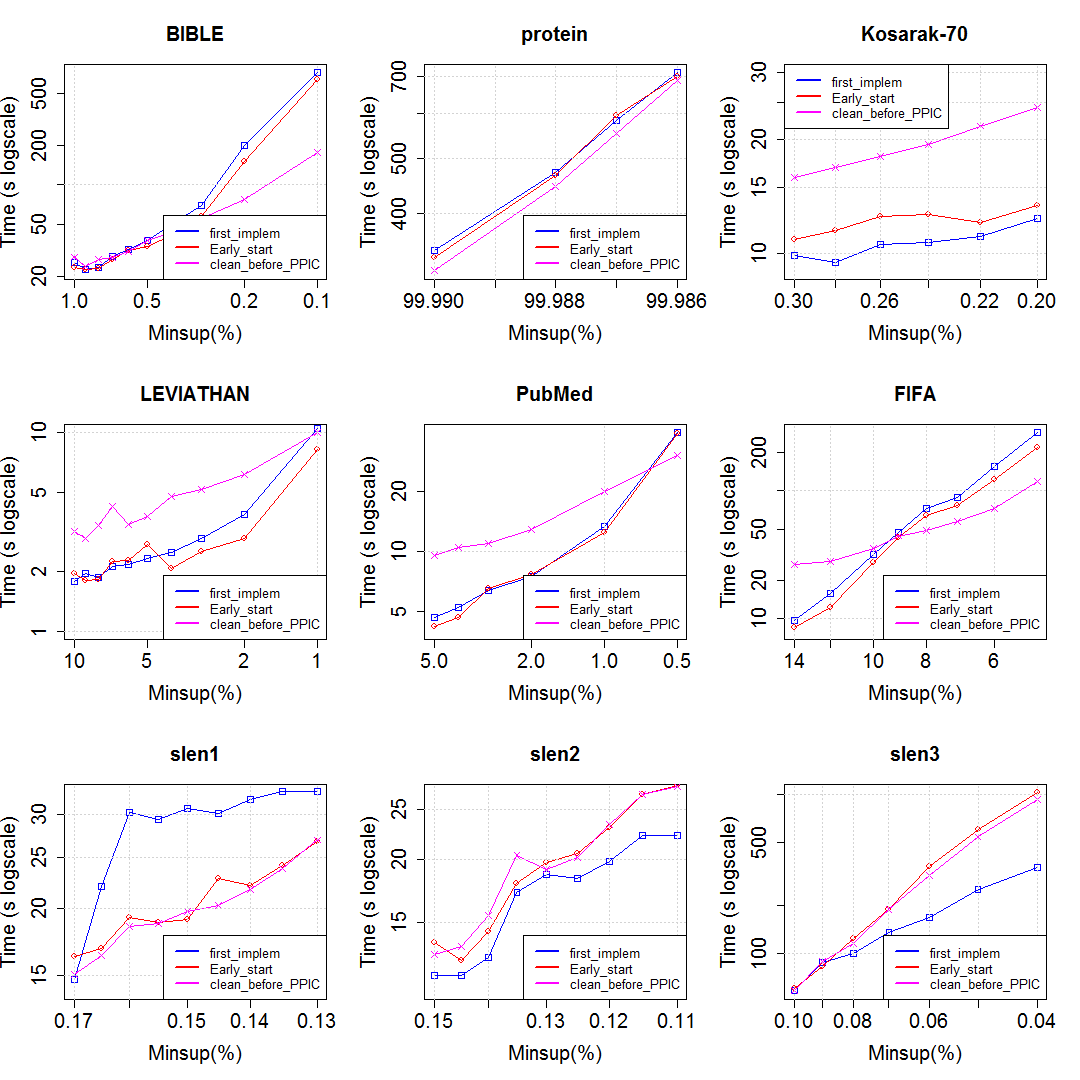
\includegraphics[width=0.9\textwidth]{new_functionalities.png}
  \caption{The performance impact of not re-calculating frequent items}
  \todo[inline]{GRAPH ONLY WITH QUICKER-START}
  \label{fig:new_functionalities_perf}
\end{figure}

As you can see, very small gain in time are generally made. At the exception of the Kosarak-70, slen2 and slen3 datasets, which are our datasets possessing the largest number of unique items after cleaning the database. At first, we believed those small loss of performance were due to the delay needed to transfer the already calculated frequent items to the various executor being larger than the time needed to actually recalculate those items from the small cleaned database. It was only much later, when we added the slen3 dataset, that we realised this interpretation was incomplete.\newline

In the original implementation, since the items need to be recalculated, they will be recalculated only on the sequences contained in the partitions of the executor. In this new version, we force every executor to receive those items and to store prefixes object for them. Those object then created will then be kept on the executor for the entirety of the execution as, should an RDD need to be recalculated, they would be a necessary input for their recreation. \newline

Meaning that, when the number of items are large, this additional feature will require more memory usage, and more computation time to received the items and their frequencies and create the prefixes. Especially when, as in our slen3 dataset which is a combination of multiple generated datasets, every partition generally concern a whole different set of items.\newline

Sadly, we realised this mistake much too late, as only the slen3 dataset proved it's quite disastrous implications and, at the time, we had decided to keep this improvement despite the small inefficiency on Kosarak and slen2. Since other datasets displayed rather interesting efficiency gain at the time. This inneficiency was thus introduced in our reference algorithm, and in nearly all the subsequent implementation. \newline

We will however correct this mistake in our final version of the algorithm, and remove the quicker-start functionality, since the change is harmful to the scalability of the program. \newline

\subsubsection{Performances of Adding Pre-processing Before PPIC's Local Execution}

\begin{figure}[h]
  \centering
  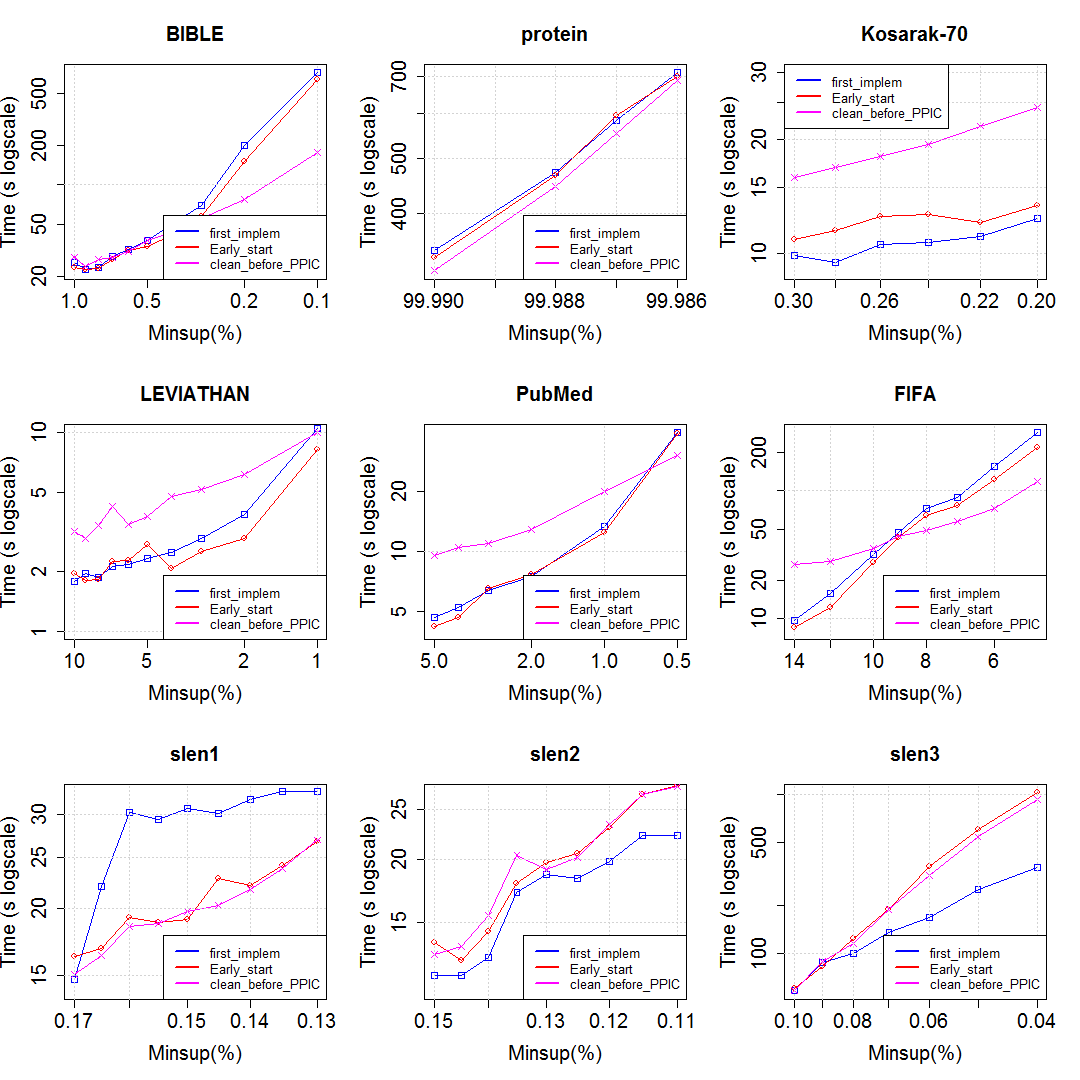
\includegraphics[width=0.9\textwidth]{new_functionalities.png}
  \caption{The performance impact of Database Pre-processing Before PPIC's Execution}
  \label{fig:clean_before_PPIC}
\end{figure}

As you can see in figure \ref{fig:clean_before_PPIC}, this additional pre-processing step allows a 3x performance speed-up on the Bible dataset and a 2x speed-up on Fifa. Lesser performance gain were also observed on protein and the latter stages of PubMed. \newline

However, we can observe worsening performances in smaller datasets and in executions with larger minsup values. Theses loss however, pales in comparison to the performance gain observed. Although at first glance they may seem large on log-scale graph, they do not even exceed ten second, while the performance can be counted in hundred of seconds on Bible and Fifa. \newline

The reason being those performance gain is that the larger the dataset and the lower the minimal amount of support, the longer prefixes will need to be before being executed locally. The larger those prefixes are before local execution, the more items can be cleaned from the sequences, the faster we can search the remain of those very sequences for patterns. Finally, if less items are present in our sequences during our local execution of PPIC, the three matrices needed for PPIC's execution can be created faster. Thus, hastening performance another fold. \newline

However, cleaning sequences comes with a variable cost depending on the database size. If, much like Kosarak, the database only contains uncleanable sequences, performances will be slightly worsened. Of course, since this change is only applied before PPIC, the performance measured on our three slen datasets weren't affected. \newline

In the end, since such large increase in performances were observed, and since so many other improvements needed to be tested, \textbf{we decided to use the performance obtained here as reference for the remainder of this paper}. To allow better comparison of performances gain/losses, all further improvement were thus added to this version, and tested separately. Finally, by the end of this paper, a final version containing all changes providing performance improvements will be compiled into a single algorithm. Of whose the performances will be tested.

\subsubsection{Performances with Automatic choice of Local Execution}

\begin{figure}[h]
  \centering
  \includegraphics[width=0.9\textwidth]{MaxItemPerItemset_recalculated.png}
  \caption[Automatic detection of item-sets type in dataset]{
  	\tabular[t]{@{}l@{}}
		Performance improvement of recalculating maxItemPerItemset to avoid \\
		search for multi-item extension when unnecessary
	\endtabular}
  \label{fig:maxItemPerItemset_recalculated}
\end{figure}

As you can see on figure \ref{fig:maxItemPerItemset_recalculated}, this improvement achieves its goal with a slight performance degradation, due to the need for calculating the maxItemPetItemSet value. \newline

While, at first, we thought those small loss where worth this additional feature, as it guarantees the use of the much more performant PPIC. We however found soon after that there was a more efficient way to achieve the same goal, as you will see in the next section.

\subsubsection{Performances of Adding Pre-processing Before Any Local Execution}

\begin{figure}[h]
  \centering
  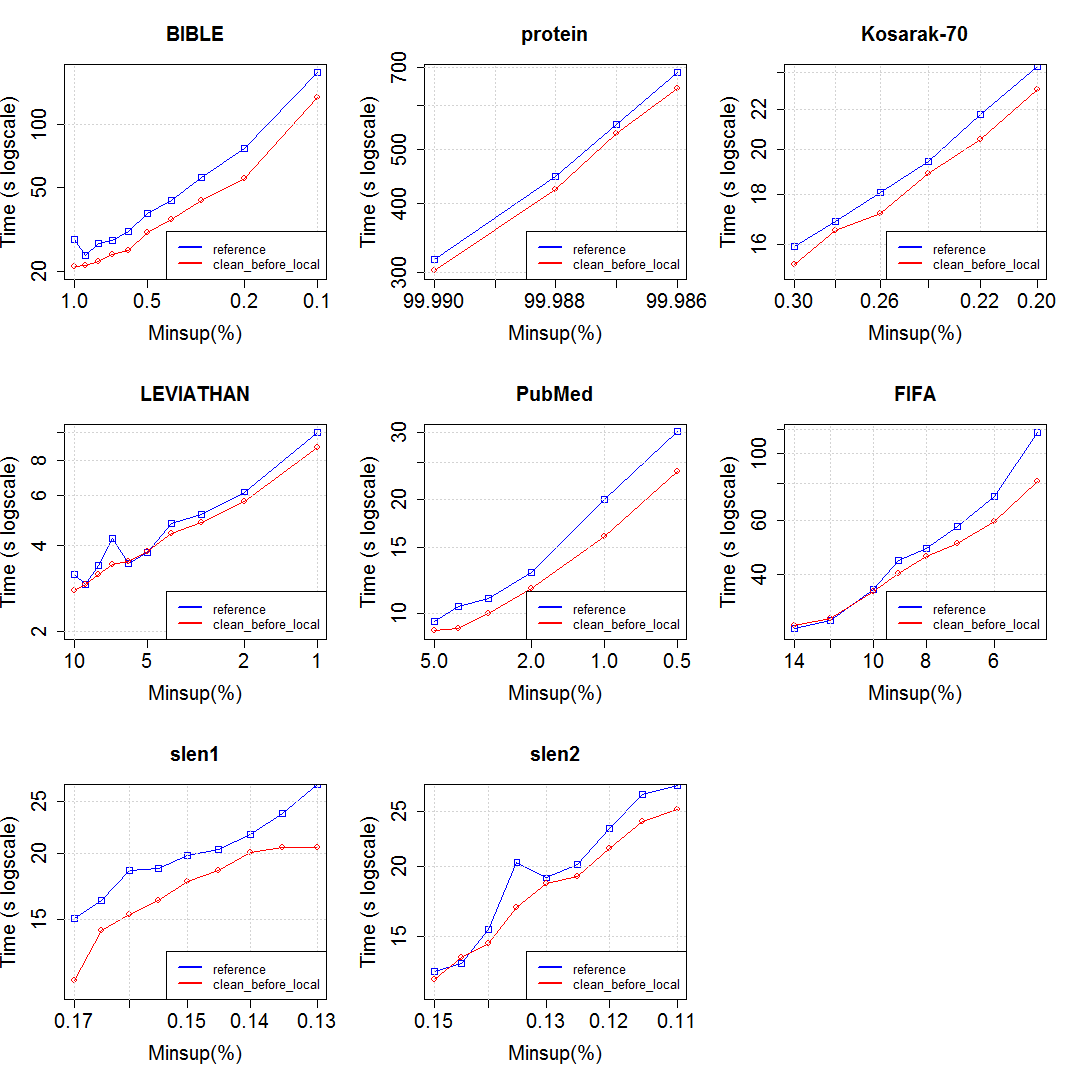
\includegraphics[width=0.9\textwidth]{clean_before_localExec.png}
  \caption{Efficiency gain of cleaning the sequence database before any local execution}
  \label{fig:cleaning_before_local_exec}
\end{figure}

As you can see in figure \ref{fig:cleaning_before_local_exec}, this implementation was, as expected, much more performant, for both types of datasets. \newline

Advantages are however lesser when mining sequences of sets of symbols, as the local execution still relies on Spark's implementation, which doesn't take much advantage of this additional cleaning step. The various improvement we made for cleaning sequence of symbols, on the other hand, are quite strongly reflected in these performance measurement, surpassing our expectation on their effectiveness.

While, as said earlier, cleaning before the local execution allows us to detect wish algorithm should take charge the the inputted database, another advantage also appeared. Should a sub-problem from a database of sequence of sets of symbol pattern become a database of sequence of symbol through cleaning, its local execution would be switched through PPIC, thus improving the significantly the performance on these projected database. \newline

Sadly those case should only appear rarely, and depend strongly on the data. Still, it remains a nice addition to have, and which give occasional small boost to performances.

\subsubsection{Performances with Position lists}

\begin{figure}[h]
  \centering
  \includegraphics[width=0.9\textwidth]{positionLists.png}
  \caption{Performance gain of first/last position lists}
  \label{fig:positionListPerf}
\end{figure}

As you can see in Figure \ref{fig:positionListPerf}, the resulting performance of those three implementation weren't conclusive. On every database of sequence of symbols but protein, which is a very sparse dataset on which this type of techniques excel, the modified algorithms delivered worse performances than our reference algorithm. \newline

Those worsening performance appear because the benefit of those additional computation simply do not have enough time to appear. After being calculated during the pre-processing step, they only stay of use during the scalable execution of our algorithm. Since that, before the local execution, the sequence database will be compressed and the positions list will need to be recalculated. \newline

Another reason for those worsening performance would be the transfer time of the calculated positions list, which can be very large depending on the number of frequent items. The delay imposed by their calculation and their transfer through the executors are thus far from negligible. \newline

However, while suffering from the same afflictions, an improvement in performance can be observed on database of sequences of sets of symbols, where those techniques weren't already in use during the local execution stage. Especially on the slen1 dataset, where performance improve significantly. \newline

However, at the exception of the slen1 dataset, the measured performance do not justify a doubled memory consumption (tripled in the case of the 'first\_last\_pos' improvement). Should no better implementation be found, the improvement could be restrained to only appear in Spark's local execution. Although performance improvement would be lesser, they would make more sense for a memory consumption point of vue.

\subsubsection{Performances with Specialized scalable execution}

\begin{figure}[h]
  \centering
  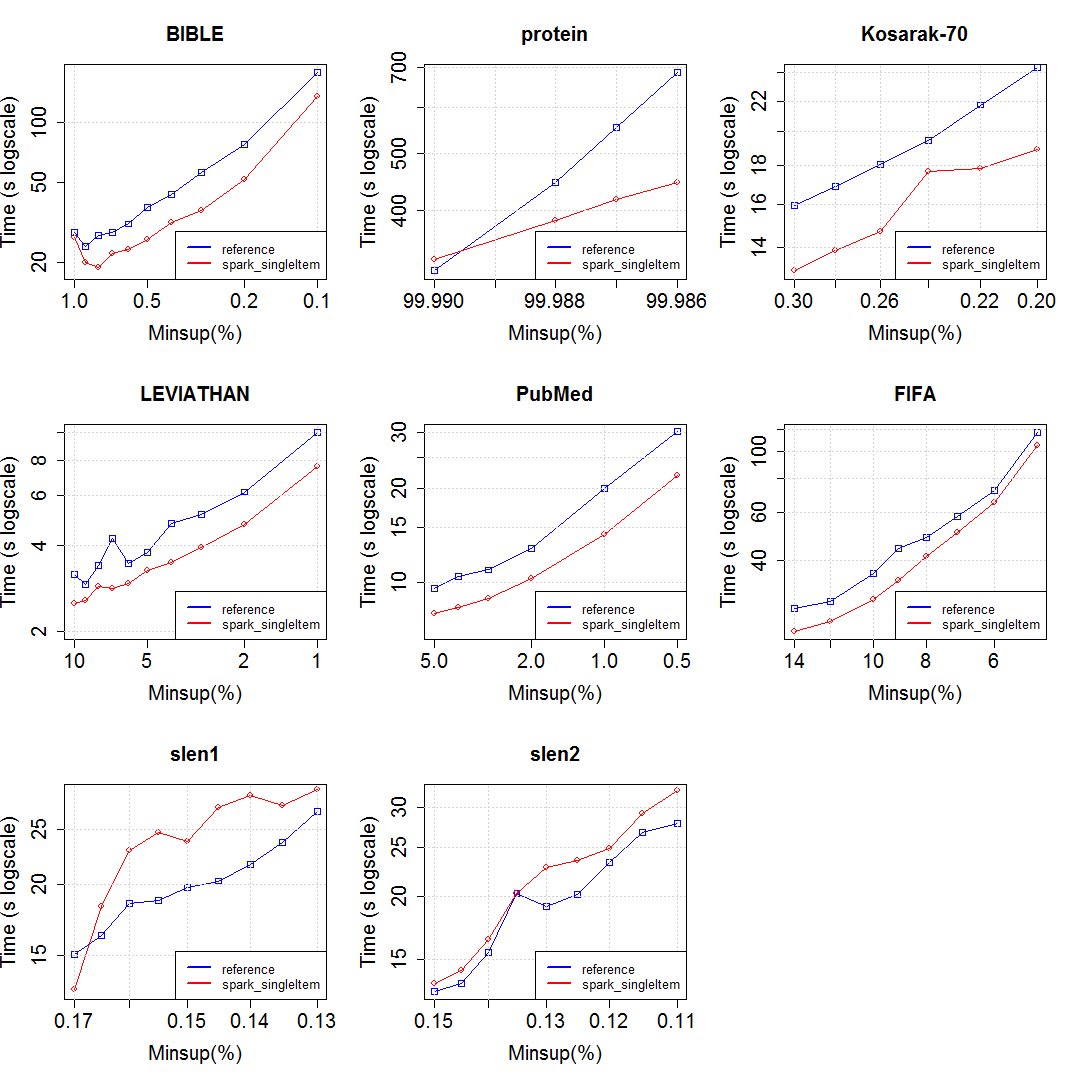
\includegraphics[width=0.9\textwidth]{scalable_single_item.png}
  \caption{Performance improvement of specialising spark's scalable stage.}
  \label{fig:scalable_single_item}
\end{figure}

As you can see on the slen datasets of Figure \ref{fig:scalable_single_item}, this improvement introduced a small loss in performance for dataset of sequence of sets of symbols. As it needs to go through the added detection but doesn't profit of the advantages. \newline

However, for sequences of symbols, performances improved greatly. Not only that, but the new internal database representation make much more sense from a memory-consumption point of view. \newline

Thus, we judged these great advantages to be worth the slight loss of performance, and decided to include this improvement in our final implementation.

\subsubsection{Performances of Using Priority Scheduling for the Local Execution}

\paragraph{Performances of Sorting Sub-Problems on the Reducer}

\begin{figure}[h]
  \centering
  \includegraphics[width=0.9\textwidth]{priority.png}
  \caption[Naive priority scheduling]{
  	\tabular[t]{@{}l@{}}
  		Performance of a 'biggest problems first' scheduling \\
  		executed through the default sortBy() function of Spark.
  	\endtabular
  }
  \label{fig:priority_scheduling_performance_comparison}
\end{figure}

As you can see in Figure \ref{fig:priority_scheduling_performance_comparison}, our first try at this implementation, impressive performance improvements can be observed, especially for the Kosarak, protein, slen2 and slen3 datasets. While BIBLE, FIFA and slen1 suffer from slight performance loss in their later stages, the damage is rather limited in comparison to the otherwise gain. Applying the sort function to the algorithm when unnecessary also isn't too damaging even when sub-problems aren't limited, as we can see with the red line, it should however be avoided in the final version. The sort function should only be called when relevant.\newline

At first glance, this thus looks like a nice little improvement. However, as explained in the implementation section, a huge problem remained. As you can see on protein's measurements, the black line lack its fourth point. The reason being a constant crash of the algorithm due to a lack of memory ! \newline

Thus motivating our second try at implementing this improvement, this time by sorting the problem on the mapper rather than the reducer.

\paragraph{Performances of Sorting Sub-Problems on the Mapper}

\begin{figure}[h]
  \centering
  \includegraphics[width=0.9\textwidth]{priority_final.png}
  \caption{Performance improvement of sorting sub-problems during map stage.}
  \label{fig:priority_scheduling_improved}
\end{figure}

This new implementation's performances were a huge success, as you can see on Figure \ref{fig:priority_scheduling_improved}. \newline

Not only have we obtained our previous boost in performance, we also avoided any memory consumption problem. This implementation advantages should thus be kept for the final version of our algorithm, since it allows far better performances when using the correct set. However, an automatic detection should be implemented, to detect when sorting sub-problems could yield increased performances, and only sort in these circumstances.

\subsubsection{Performances of using a Map Based Sequence Database Structure}

\begin{figure}[h]
  \centering
  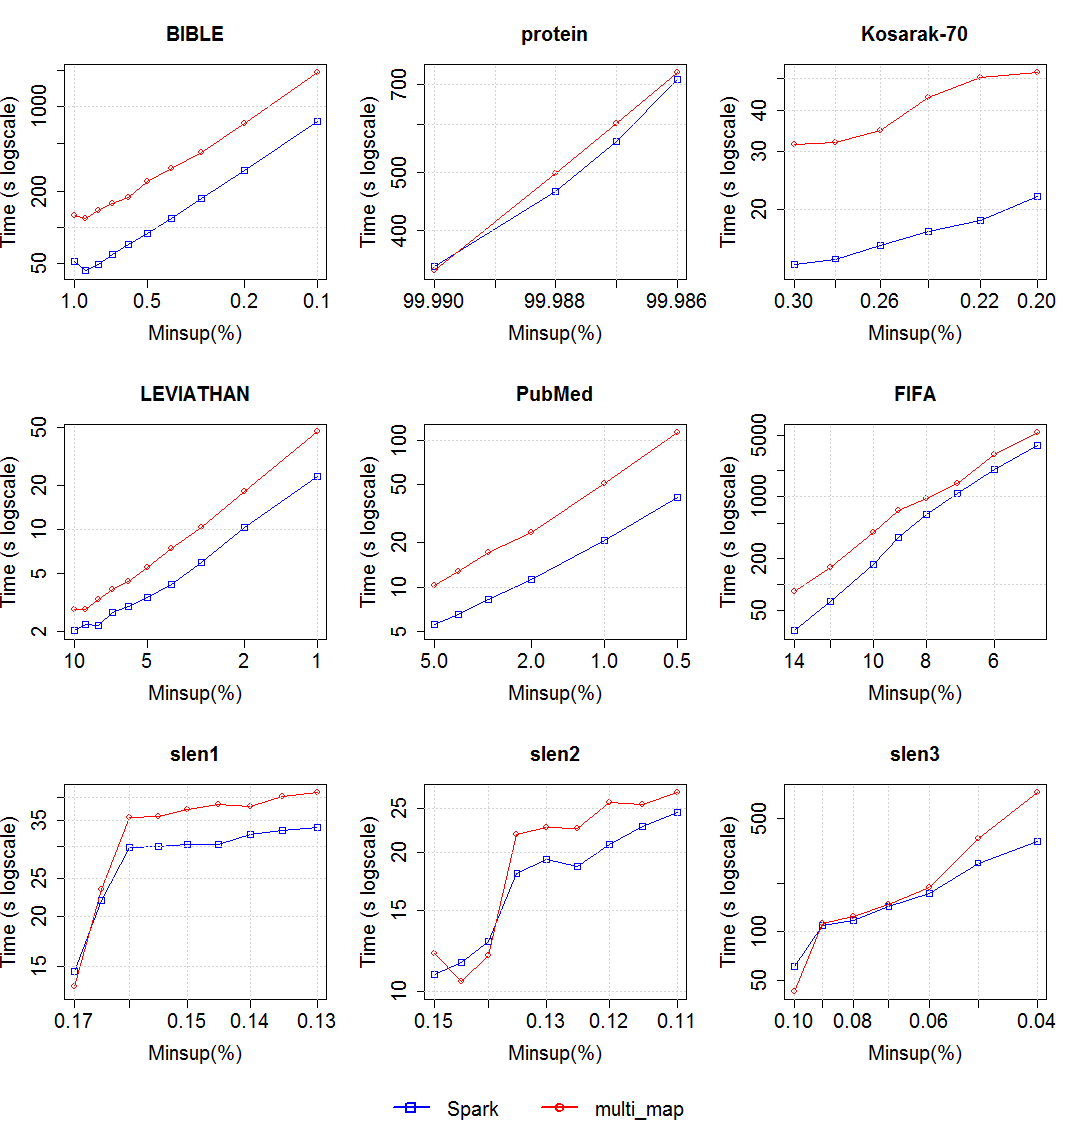
\includegraphics[width=0.9\textwidth]{multi_item_map.png}
  \caption[Map based - multi\_item algorithm]{
  	\tabular[t]{@{}l@{}}
  		Performance of a CP based algorithm replacing \\
  		all three pre-processed matrices from PPIC by a Map structure
  	\endtabular
  }
  (Please take notice that we are here comparing to the original Spark implementation instead of the reference algorithm. Since the featured implementation doesn't posses the early-start improvement and the comparison is, in this case, much more relevant.)
  \label{fig:multi_map}
\end{figure}

As you can see in Figure \ref{fig:multi_map}, the performance of this implementation were terrible. \newline

Profiling our algorithm revealed it came from two majors factor. First, as feared, to attain the same purpose as the three matrices with our map structure, we needed many more trailing points which had to be backtracked at each step of the search. Regularly generating significant period of time were our algorithm did nothing but backtrack the various sequences of its database. \newline

The second factor was solution pruning. In PPIC, pruning our search space could be done by checking the last positions of each item, quickly asserting that if the start of a sequence was after the last position of an item in a sequence, the sequence was no longer supporting the item. \newline

Here, however, the situation is different. To efficiently prune a multi-item pattern problem, checking last positions was no longer sufficient. To prune efficiently, each itemSet now needs to be checked so that its possible extensions could be deemed supported. \newline

Which amount to this algorithm doing twice the work for the same results. As we found out through our tests, pruning using PPIC's original method (last position list) instead of fully, as spark did, produces better performance. A comparison of the two being available in the annexes, figure \ref{fig:multi_map_comp}. \newline

Although the performance are better when not fully pruning our search space. Spark's original local execution was still much more efficient.

\subsubsection{Performances PPIC with Partial Projection}

\begin{figure}[h]
  \centering
  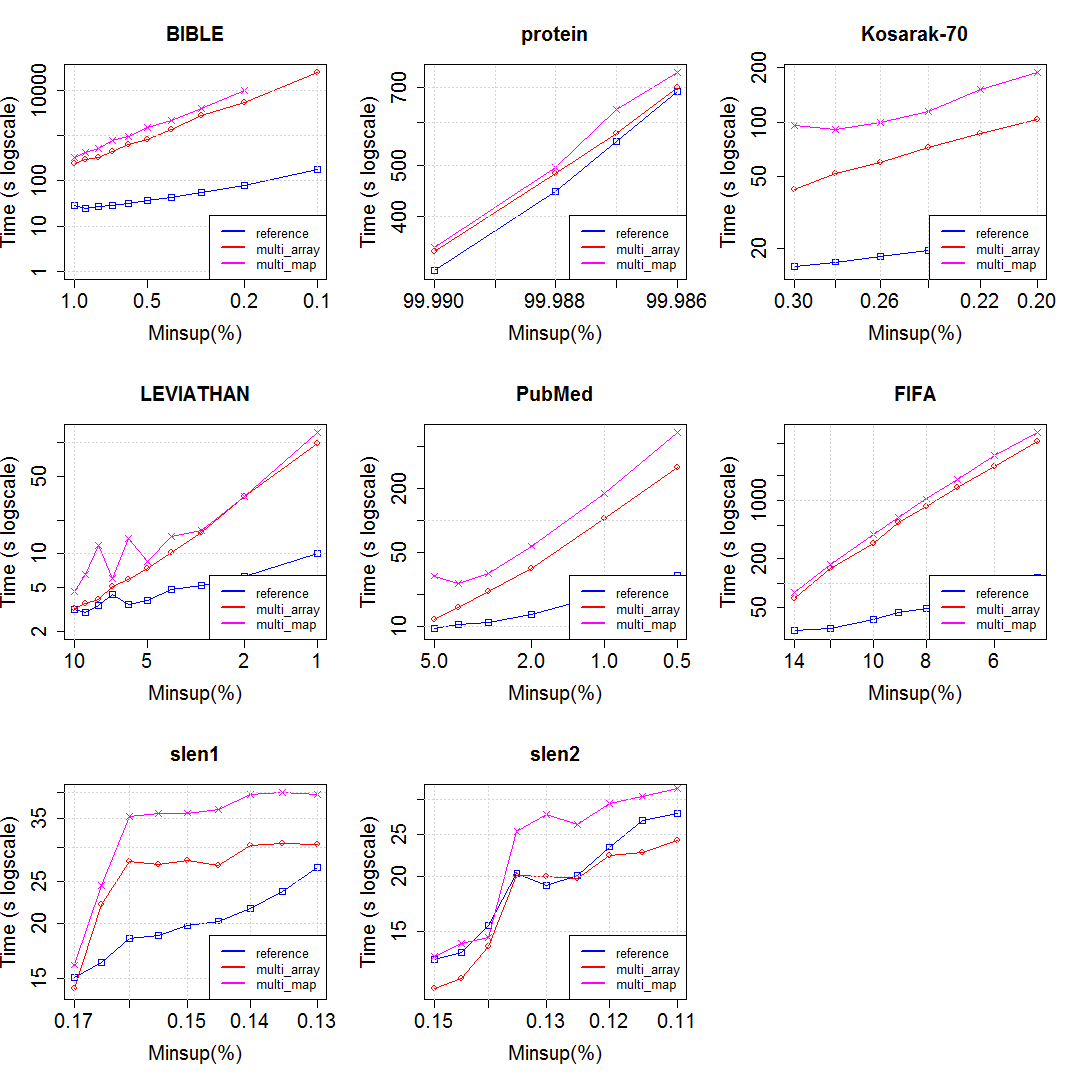
\includegraphics[width=0.9\textwidth]{multi_item_cp.png}
  \caption[PPIC with partial starts]{
  	\tabular[t]{@{}l@{}}
  		Performance of a CP based algorithm extending \\
  		PPIC's implementation by maintaining partial starts.
  	\endtabular
  }
  \label{fig:multi_array}
  (Please take notice that we are here comparing to the original Spark implementation instead of the reference algorithm. Since the featured implementation doesn't posses the early-start improvement and the comparison is, in this case, much more relevant.)
\end{figure}

The performance tests realised at the end of our implementation, shown in figure \ref{fig:multi_array}, revealed improved efficiency in comparison to spark original algorithm and our previously created map algorithm on sequence of sets of symbols. On slen3, this implementation was even much more efficient than anything obtained earlier through positions lists. \newline

These performance however came at the cost of an inefficiency on dataset of sequences of symbols, where performances fails to overcome spark's standard on anything but the FIFA dataset. \newline

This implementation should thus only be used for dealing with sets of symbols, while sequence of symbols should be found through PPIC, whose efficiency was focused on this kind of problem.

\subsection{Scalability Tests}

\section{Conclusion}

\clearpage
TODO - ADD REFERENCES, CA MANQUE ENCORE
\nocite{*}
\addcontentsline{toc}{section}{References}
\bibliographystyle{ieeetr}
\bibliography{ref}

\clearpage
\section{Annexes}

\subsection{Glossary :}

\printglossary[type=\acronymtype]

\subsection{Additional example images}

\begin{figure*}[h]
  \centering
  \begin{subfigure}[t]{0.5\textwidth}
  	\centering
    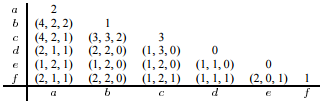
\includegraphics[width=1\textwidth]{Smatrix.png}
    \caption{S-matrix in original database}
  \end{subfigure}
  \begin{subfigure}[t]{0.49\textwidth}
  	\centering
    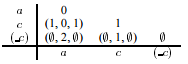
\includegraphics[width=0.6\textwidth]{SabMatrix.png}
    \caption{S-matrix in <AB>-projected database}
  \end{subfigure}
  \vspace{5px} \\
  S-M[a, b] = (4, 2, 2) => support(AB) = 4; support(BA) = 2; support((AB)) = 2;
  \caption{Example of an S-matrix for Prefix-Span bi-level projection}
  \label{fig:smatrix}
\end{figure*}

\subsection{Additional Performance Comparisons :}

\begin{figure}[h]
  \centering
  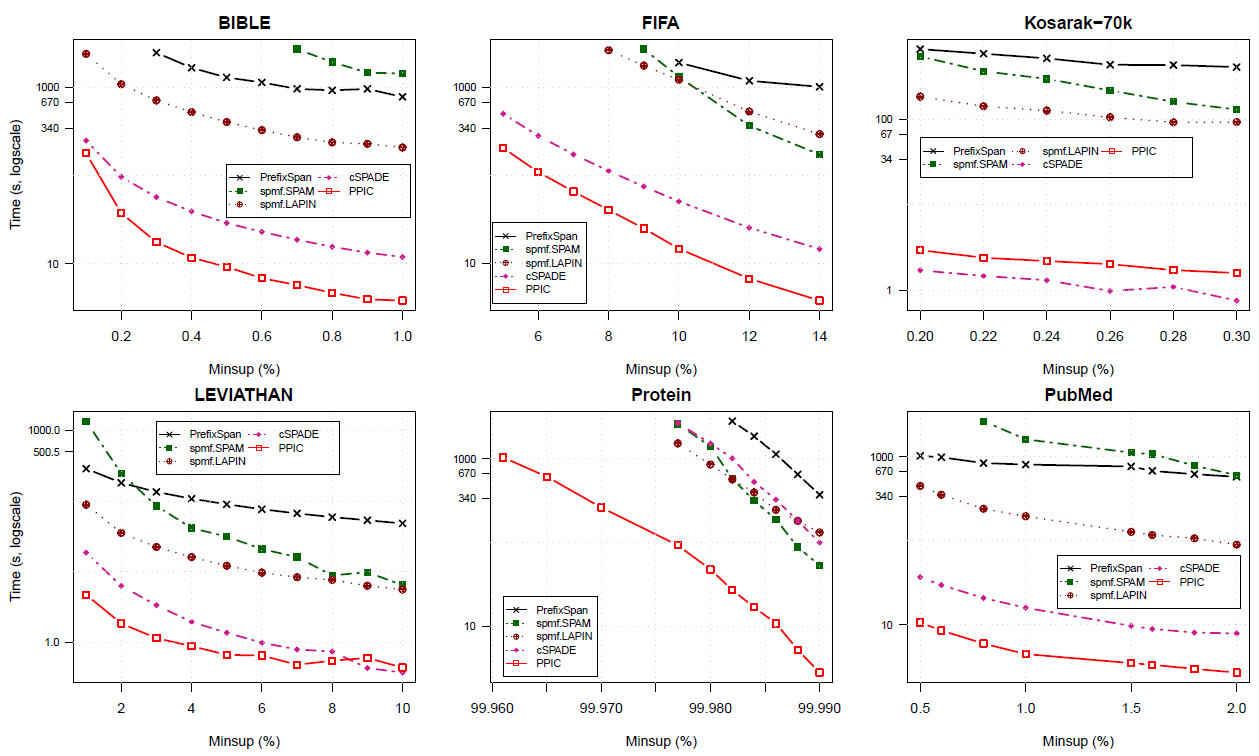
\includegraphics[width=1\textwidth]{PPICvsSpecialised.png}
  \caption{PPIC's performances VS other specialized algorithm}
  \label{fig:PPICvsOther}
\end{figure}

\begin{figure}[h]
  \centering
  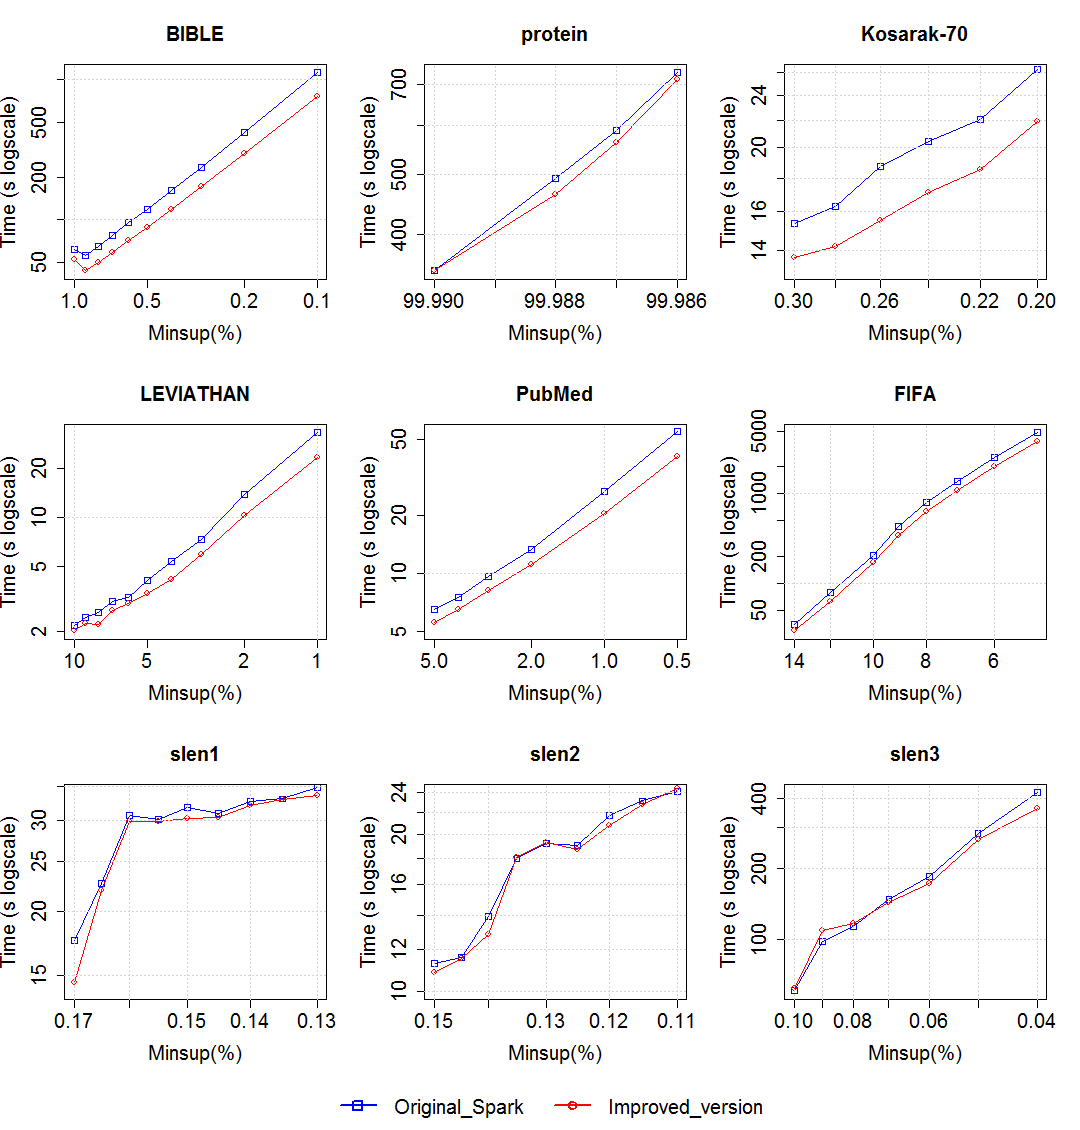
\includegraphics[width=0.9\textwidth]{spark_original_fixed_preprocessing.png}
  \caption{Performance improvement of fixing Spark's pre-processing}
  \label{fig:spark_preprocessing_fix}
\end{figure}

\begin{figure}[h]
  \centering
  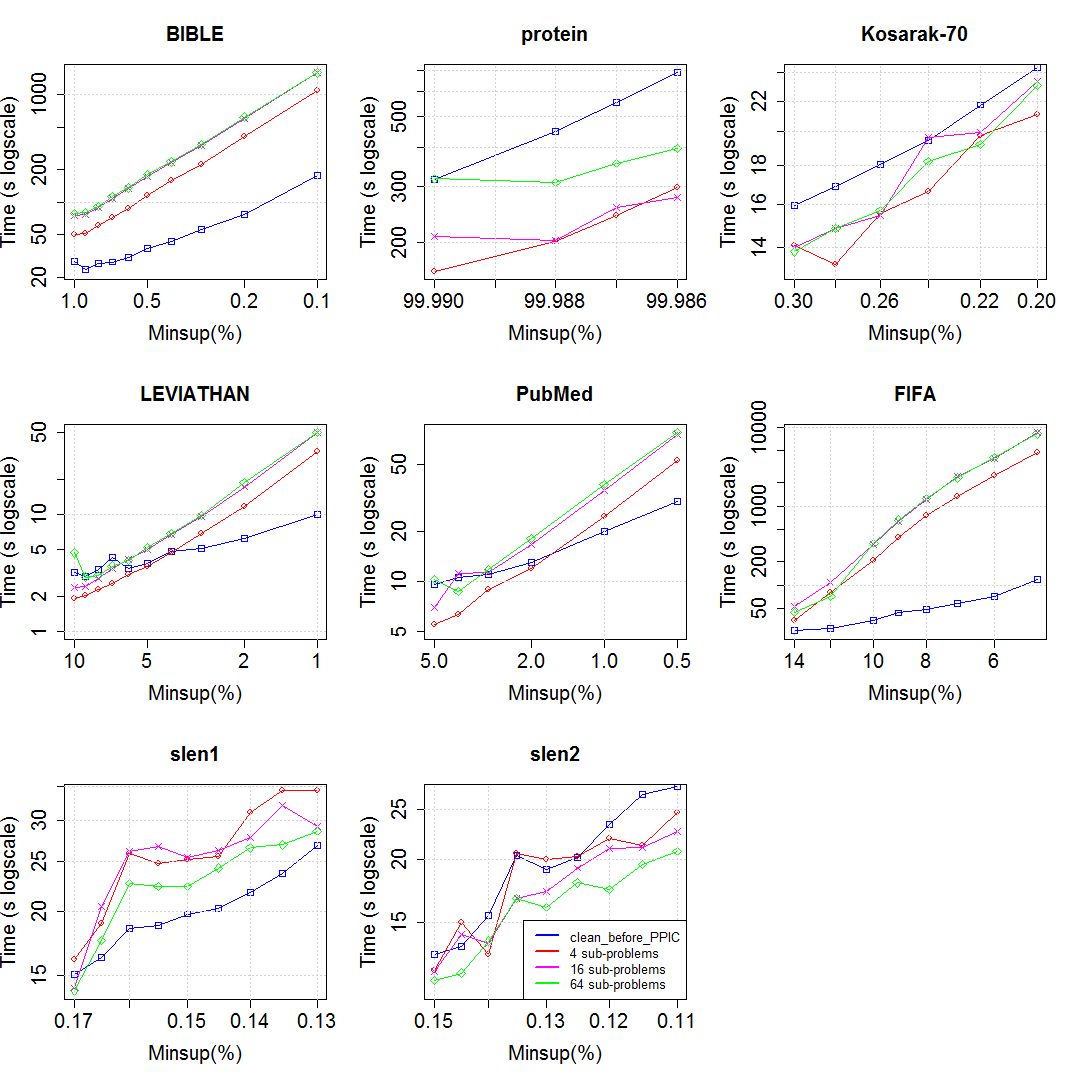
\includegraphics[width=0.9\textwidth]{sub_problem_limit.png}
  \caption[Performance improvement - soft limit on the number of created sub-problem.]{
  	\tabular[t]{@{}l@{}}
  		Performance improvement - soft limit on the number of created sub-problem. \\ 
  		Tested on the reference (Clean Before Local Exec) implementation.
  	\endtabular
  }
  (P
  \label{fig:sub_problem_limit}
\end{figure}

\begin{figure}[h]
  \centering
  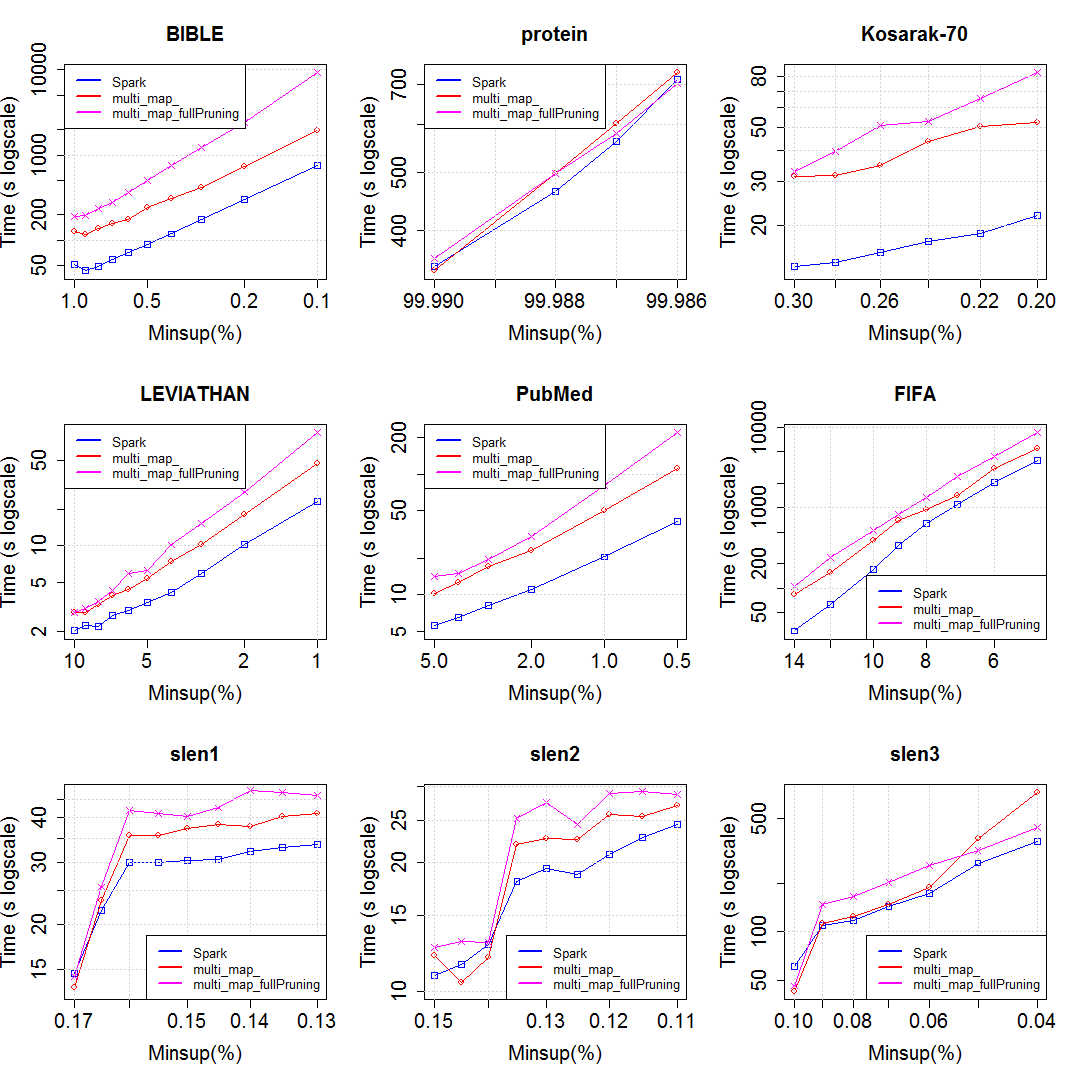
\includegraphics[width=0.9\textwidth]{multi_item_map_improved.png}
  \caption[PPIC with a map structure]{
  	\tabular[t]{@{}l@{}}
  		Performance comparison of a full pruning VS a partial pruning \\ 
  		on the \textrm{multi\_map} implementation.
  	\endtabular
  }
  (Please take notice that we are here comparing to the original Spark implementation instead of the reference algorithm. Since the featured implementation doesn't posses the early-start improvement and the comparison is, in this case, much more relevant.)
  \label{fig:multi_map_comp}
\end{figure}

\clearpage
\subsection{Algorithms :}

\RestyleAlgo{boxruled}
\LinesNumbered
\begin{algorithm}[h]
	\caption{Prefix Projection Incremental Counting propagator (PPIC)}
    \label{alg:PPIC1}
  
    \KwData{Given a sequence of symbol database (SDB), an array of reversible int representing our search space (P), and minimal number of support ($\theta$)}
    \KwResult{PPIC return the set of frequent sequence of symbol contained in SDB, such that any returned pattern appear at least $\theta$ times in the database.}
    
    \SetKwProg{Fn}{Function}{ :}{end}
    \SetKwFunction{Propagate}{propagate}

	\tcp{Init global param :}
	sids = [0, ..., len(SDB)]; poss = [0] * len(SDB); \\
	$\phi = 0$; $\varphi = len(SDB)$ \\
	projFreq = Array such that projFreq[i] contains the number of sequence initially supporting symbol i; \\
	\Fn{\Propagate{$SDB,P,i,\theta$}} {
		\tcp{espilon == special value that ends a valid pattern}
    	\uIf {$P_i$ isBoundTo(epsilon)} {
    		\tcp{A valid pattern has been found, fill remaining space to collect}
    		\tcp{$P_0$ cannot be bound to epsilon}
    	 	\ForEach {j in ${i+1, ..., L}$} {P(j).assign(epsilon)}
    	 	\tcc{When success is returned, the current pattern is collected a solution and we backtrack to the previous node of the search tree.}
    	 	\Return Success
    	}
    	\Else { 
    		\While {$P_i$ isBound and i < len(P)} {
    	 		nSupport = projectAndGetFreqs($SDB, Pi, \theta, sids, poss, \phi, \varphi$) \\
    	 		\If {nSupport < $\theta$} {
    	 			\tcc{When failure is returned, we backtrack to the previous node of the search tree.}
    	 			\Return Failure
    	 		}
    	 		\tcp{projFreq has been updated by the projectAndGetFreqs method.}
    	 		\tcp{Prune domain of $P_{i+1}$}
    	 		pruneDomain($i+1, projFreq$) \\
    	 		i++
    	 	}
    	}
    	\tcc{When suspend is returned, we continue down the search tree.}
    	\Return Suspend
   	}
\end{algorithm}

\RestyleAlgo{boxruled}
\LinesNumbered
\begin{algorithm}[h]
	\caption{PPIC Continued}
    \label{alg:PPIC2}
    
    \SetKwProg{Fn}{Function}{ :}{end}
    \SetKwFunction{Proj}{projAndGetFreqs}
    
   	\Fn{\Proj{$SDB, itemToProject, \theta, sids, poss, \phi, \varphi$}} {
   		projFreq[a] = 0   $\forall a \in \{ 1, ..., nSymbols \}$ \\
   		i = $\phi$; j = $\phi + \varphi$; sup = 0 \\
   		\While{$i < \phi + \varphi$}{
   			sid = sids[i]; pos = poss[i]; seq = SDB[sid] \\
   			\tcc{pos => first position in  a sequence, such that the previous prefix was supported. To project the new item, we only need to search the remains of the sequence.}
   			\tcc{sid => The sequence id of a sequence which supported the previous prefix.}
   			\tcc{sids => A vector starting at position $\phi$ and containing $\varphi$ elements, allowing to only search sequence that supported the previous pattern.}
   			\tcc{seq => A sequence where the new item should be projected.}
   			\If {lastPosMap(sid)(itemToProject) - 1 > pos} {
   				\tcp{Find next position of itemToProject in seq}
   				\uIf {pos < firstPosMap(sid)(itemToProject)} {
   					\tcp{Jump to first occurrence of the item in the sequence}
   					pos = firstPosMap(sid)(itemToProject)
   				}
   				\Else {
   					\tcp{Search for the next position of itemToProject}
   					\While {pos < len(seq) and itemToProject != seq[pos]} {
   						pos = pos + 1
   					}
   				}
   				\tcp{item supported -> update projected database}
				sids[j] = sid; poss[j] = pos + 1; j = j + 1; sup = sup + 1; \\
				posToCheck = interestingPosMap(sid)(pos)
				\While {$posToCheck != 0$} {
					\tcp{Faster than checking lastPosMap}
					symbol = seq[posToCheck - 1]
					projFreqs[symbol] = projFreqs[symbol] + 1
					posToCheck = interestingPosMap(sid)(posToCheck - 1)
				}
   			}
   			i = i+1
   		}
   		$\phi$ = $\phi + \varphi$; $\varphi$ = sup \\
		return projFreqs
   	}
\end{algorithm}

\RestyleAlgo{boxruled}
\LinesNumbered
\begin{algorithm}[h]
	\caption{Spark's original implementation : Pre-Processing}
    \label{alg:SPARK1}
  
    \KwData{Given a sequence of sets of symbol database (SSDB), a minimal number of supporting sequence ($\theta$), a maximal pattern length (maxPatLen), and a maximal local projected database size (maxLocalSize)}
    \KwResult{Return the set of frequent sequence of sets of symbol contained in SDB. Such that any returned pattern appear at least $\theta$ times in the database.}
    
    \SetKwProg{Fn}{Function}{ :}{end}
    \SetKwFunction{Pre}{PreProcessing}

	\Fn{\Pre{$SSDB, maxPatLen, maxLocalSize, \theta$}} {
		\tcp{Clean database through a map reduce phase}
    	freqItems = findFrequentItem(SSDB, $\theta$) \\
    	cleanedSequences = cleanSequenceAndRenameItem(SSDB, freqItems)\\
    	\tcp{Find frequent sequences of sets of symbols}
    	solutionPatterns = scalableExecution(cleanedSequences, maxPatLen, maxLocalSize, $\theta$) \\
    	\tcp{Translate to original items name and Return}
    	\Return translateBackToOriginalItemsName(solutionPatterns)
   	}
\end{algorithm}

\RestyleAlgo{boxruled}
\LinesNumbered
\begin{algorithm}[h]
	\caption{Spark's original implementation : Scalable execution}
    \label{alg:SPARK2}
    
    \SetKwProg{Fn}{Function}{ :}{end}
    \SetKwFunction{Scalable}{scalableExecution}
    
   	\Fn{\Scalable{$SSDB, maxPatLen, maxLocalSize, \theta$}} {
		\tcc{Encapsulate each sequence in a postfix, allowing to keep the current position and partial starts without copying the sequences.}
		postfixes = SSDB.map(seq => PostFix(seq)) \\
		\tcp{Init prefix list and solution list}
		solutionPatterns = Array.empty \\
		smallPrefixes = Array.empty \\
		largePrefixes = [prefix.empty] \\
		\tcp{Start scalable execution}
		\While {largePrefixes is not empty}{
			mapReduceResults = postifixes.flatMap( postfix => \\
				\Indp
				largePrefixes.flatMap( prefix => \\
					\Indp
					extensions = postfix.project(prefix).findPrefixExtension()\\
					extensions.map( (item, postfixSize) => \\
						\Indp
						\tcp{Return a (key, value) pair}
						((prefix.id, item), (1, postfixSize)) \\
						\Indm
					) \\
					\Indm
				) \\
				\Indm
			).reduceByKey($(v1.1 + v2.1, v1.2 + v2.2)$) \tcp{Aggregate values by key}
			.filterByValue($v.1 \geq \theta$) \tcp{Keep key-value pair with enough support}
			\tcp{Empty larger prefixes list}
			largePrefixes.clean()\\
			\tcp{Fill it with new, extended, prefixes}
			\ForEach{((prefiID, extendingItem), (support, projDBSize) $\in$ mapReduceResults}{
				\tcp{Create prefix, add it as solution}
				newPrefix = largePrefixes.getByID(prefixID) += extendingItem \\
				solutionPatterns += newPrefix \\
				\If {len(newPrefix) < maxPatternLength}{
					\tcp{len(newPrefix) == number of non-zero item in prefix}
					\tcp{zero == separator between itemSets}
					\uIf {projDBSize > maxLocalProjDBSize} {
              			largePrefixes += newPrefix
            		} 
            		\Else {
              			smallPrefixes += newPrefix
            		}
				} 
			}
		}
		\If {len(smallPrefixes) > 0} {
			\tcp{For each prefix, project the whole database and solve locally}
			toExecuteLocaly = postifixes.flatMap( postfix => \\
				\Indp
				smallPrefixes.flatMap( prefix => \\
					\Indp
					(prefix.ID, postfix.project(prefix).compress())\\
					\Indm
				)\\
				\Indm
			).groupByKey().flatMap(sequences => \\
				\Indp
				localExecution(sequences, maxPatLen - len(prefix), $\theta$) \\
				\Indm
			) \\
		}
   	}
\end{algorithm}

\RestyleAlgo{boxruled}
\LinesNumbered
\begin{algorithm}[h]
	\caption{Spark's original implementation : Local execution}
    \label{alg:SPARK3}
    
    \SetKwProg{Fn}{Function}{ :}{end}
    \SetKwFunction{Local}{localExecution}
    
   	\Fn{\Local{$SSDB, maxPatLen, \theta$}} {
   		\If {maxPatLen == 0}{\Return Array.empty}
   		\tcp{Find extending item that are sufficiently frequent}
   		counts = Map[Int, Int].empty.withDefaultValue(0) \\
		\ForEach {postfix $\in$ SSDB} {
			\ForEach {(extendingItem, size) $\in$ postfix.findPrefixExtension()} {
				counts(extending) += 1
			}
		}
		counts = counts.filterByValue(val $\geq \theta$) \\
		\tcp{Extend for each item and continue searching}
		solutions = ArrayList.empty[Prefix] \\
		\ForEach {key $\in$ counts} {
			projectedDB = postfixes.project(key)\\
			\ForEach {extension $\in$ localExecution(projectedDB, maxPatLen-1, $\theta$)}{
				solution += key + extensions
			}
		}
		\Return solutions
   	}
\end{algorithm}

\RestyleAlgo{boxruled}
\LinesNumbered
\begin{algorithm}[h]
	\caption{Spark's original implementation : Project and findPrefixExtension}
    \label{alg:SPARK4}
    
    \SetKwProg{Class}{Class}{ :}{end}
    \SetKwProg{Fn}{Function}{ :}{end}
    \SetKwFunction{Postfix}{Postfix}
    \SetKwFunction{Project}{project}
    
   	\Class{\Postfix{$sequence$}} {
   	
   		start = 0 \\
   		partialProjections = Array.empty
   		
   		\Fn{\Project(Item)} {
   			\If {start > len(sequence)} {\Return}
   			newPartialProjection = Array.empty \\
   			\uIf {Item extends current ItemSet in Prefix} {
   				\ForEach {partial $\in$ partialProjections} {
   					newPos = findNextItemInCurrentItemSet(sequence, partial, Item) \\
   					\If {Found Item in current ItemSet}{
   						newPartialProjection += newPos
   					}
   				}
   				start = findSmallestPosition(newPartialProjection) + 1 \\
   			} 
   			\ElseIf {Item start a new ItemSet in Prefix} {
   				\For {Pos $\in \{start, ..., len(sequence) - 1\}$}{
   					\If {sequence[Pos] == Item} {
   						\uIf {first found in loop} {
   							start = Pos + 1
   						}
   						\Else {
   							newPartialProjection += Pos
   						}
   					}
   				}
   			}
   			partialProjections = newPartialProjection
   		}
   		\Fn{\Project(Prefix)} {
   			\ForEach {Item $\in$ Prefix} {
   				this.project(Item)
   			}
   		}
   		\Fn{\Project(findPrefixExtension)} {
   			extendingItems = Set.empty \\
   			\ForEach {partial $\in$ partialProjections} {
   				\tcp{Find items that extend current itemSet}
   				extendingItems ++= findAllItemUntilNextSeparator(sequence, partial)
   			}
   			\For {Pos $\in \{start, ..., len(sequence) - 1\}$}{
   				\tcp{Find items that start a new itemSet}
   				extendingItems += sequence[Pos]
   			}
   		}
   	}
\end{algorithm}

\RestyleAlgo{boxruled}
\LinesNumbered
\begin{algorithm}[h]
	\caption{First scalable CP based implementation}
    \label{alg:FirstImplem}
    
    \SetKwProg{Fn}{Function}{ :}{end}
    \SetKwFunction{Scalable}{scalableExecution}
    
   	\Fn{\Scalable{$SSDB, maxPatLen, maxLocalSize, \theta, hasSetsOfSymbols$}} {
		\tcc{Encapsulate each sequence in a postfix, allowing to keep the current position and partial starts without copying the sequences.}
		postfixes = SSDB.map(seq => PostFix(seq)) \\
		\tcp{Init prefix list and solution list}
		solutionPatterns = Array.empty \\
		smallPrefixes = Array.empty \\
		largePrefixes = [prefix.empty] \\
		\tcp{Start scalable execution}
		\While {largePrefixes is not empty}{
			... \tcp{Same as Spark's original implementation}
		}
		\tcp{Start local execution}
		\If {len(smallPrefixes) > 0} {
			\tcp{For each prefix, project the whole database and solve locally}
			toExecuteLocaly = postifixes.flatMap( postfix => smallPrefixes.flatMap( prefix => \\
					\Indp
					(prefix.ID, postfix.project(prefix).compress())\\
					\Indm
			)).groupByKey().flatMap(sequences => \\
				\tcp{Use argument to determine which local execution to use}
				\uIf {hasSetsOfSymbols} {
					localExecution(sequences, maxPatLen - len(prefix), $\theta$) \\
				}
				\Else {
					sequences = removeSeparator(sequences) \\
					matrices = generatePPICMatrices() \\
					\tcc{PPIC will generate the P vector, add constraint to enforce maxPatLen and then launch the execution, calling propagate in the process.}
					PPIC(sequences, maxPatLen - len(prefix), $\theta$, matrices) \\
				}
			) \\
		}
   	}
\end{algorithm}

\RestyleAlgo{boxruled}
\LinesNumbered
\begin{algorithm}[h]
	\caption{New functionalities : Scalable execution}
    \label{alg:NF}
    
    \SetKwProg{Fn}{Function}{ :}{end}
    \SetKwFunction{Scalable}{scalableExecution}
    
   	\Fn{\Scalable{$SSDB, minPatLen, maxPatLen, maxLocalSize, \theta,$ \\ $limitItemPerItemset, softSubProblemLimit$}} {
		\tcc{Encapsulate each sequence in a postfix, allowing to keep the current position and partial starts without copying the sequences.}
		postfixes = SSDB.map(seq => PostFix(seq)) \\
		\tcp{Init prefix list and solution list}
		solutionPatterns = Array.empty \\
		smallPrefixes = Array.empty \\
		largePrefixes = [prefix.empty] \\
		\tcp{Start scalable execution}
		\While {largePrefixes is not empty}{
			\If {len(largePrefixes) + len(smallPrefixes) $\geq$ softSubProblemLimit > 0} {
				smallPrefixes ++= largePrefixes \tcp{Switch to local execution}
				break
			}
			mapReduceResults = postifixes.flatMap( postfix => \\
				\Indp
				... \tcp{See First Scalable CP based Implementation}
				\Indm
			).reduceByKey($(v1.1 + v2.1, v1.2 + v2.2)$) \tcp{Aggregate values by key}
			.filterByValue($v.1 \geq \theta$) \tcp{Keep key-value pair with enough support}
			\tcp{Empty larger prefixes list}
			largePrefixes.clean()\\
			\tcp{Fill it with new, extended, prefixes}
			\ForEach{((prefiID, extendingItem), (support, projDBSize) $\in$ mapReduceResults}{
				\tcp{Create prefix, add it as solution}
				newPrefix = largePrefixes.getByID(prefixID) += extendingItem \\
				\If {respectConstraints(newPrefix, minPatLen, limitItemPerItemset)}{
					solutionPatterns += newPrefix 
				}
				\If {canExtendedItemRespectConstraint(newPrefix, maxPatLen, limitItemPerItemset}{
					\tcp{Search extensions for this prefix}
					\uIf {projDBSize > maxLocalProjDBSize} {
              			largePrefixes += newPrefix
            		} 
            		\Else {
              			smallPrefixes += newPrefix
            		}
				} 
			}
		}
		\If {len(smallPrefixes) > 0} {
			\tcc{Similar local execution than in First Scalable CP based Implementation, but with additional checks to guarantee that the new constraints are respected.}
			...
		}
   	}
\end{algorithm}

\RestyleAlgo{boxruled}
\LinesNumbered
\begin{algorithm}[h]
	\caption{Quick - Start : Scalable execution}
    \label{alg:QuickStart}
    
    \SetKwProg{Fn}{Function}{ :}{end}
    \SetKwFunction{Scalable}{scalableExecution}
    
   	\Fn{\Scalable{$SSDB, minPatLen, maxPatLen, maxLocalSize, \theta,$ \\ $limitItemPerItemset, softSubProblemLimit, frequentItemAndCount$}} {
		\tcc{Encapsulate each sequence in a postfix, allowing to keep the current position and partial starts without copying the sequences.}
		postfixes = SSDB.map(seq => PostFix(seq)) \\
		\tcp{Init prefix list and solution list}
		solutionPatterns = Array.empty \\
		smallPrefixes = Array.empty \\
		largePrefixes = Array.empty \\
		\ForEach {(item, count) $\in$ frequentItemAndCount} {
			largePrefixes += Prefix(item, count) \tcp{count == nbSupport for item}
		}
		\tcp{Start scalable execution}
		\While {largePrefixes is not empty}{
			\tcp{Project and extend prefix}
		}
		\If {len(smallPrefixes) > 0} {
			\tcp{Project and extend prefix locally}
		}
   	}
\end{algorithm}

\RestyleAlgo{boxruled}
\LinesNumbered
\begin{algorithm}[h]
	\caption{Clean database before local execution of PPIC :}
    \label{alg:CleanBeforeLocalPPIC}
    
    \SetKwProg{Fn}{Function}{ :}{end}
    \SetKwFunction{Scalable}{scalableExecution}
    
   	\Fn{\Scalable{$SSDB, minPatLen, maxPatLen, maxLocalSize, \theta,$ \\ $hasSetsOfSymbols, limitItemPerItemset, softSubProblemLimit, freqItemAndCount$}} {
		\tcc{Encapsulate each sequence in a postfix, allowing to keep the current position and partial starts without copying the sequences.}
		postfixes = SSDB.map(seq => PostFix(seq)) \\
		\tcp{Init prefix list and solution list}
		solutionPatterns = Array.empty \\
		smallPrefixes = Array.empty \\
		largePrefixes = Array.empty \\
		\ForEach {(item, count) $\in$ freqItemAndCount} {
			largePrefixes += Prefix(item, count)\tcp{count == nbSupport for item}
		}
		\tcp{Start scalable execution}
		\While {largePrefixes is not empty}{
			\tcp{Project and extend prefix}
		}
		\If {len(smallPrefixes) > 0} {
			\tcp{For each prefix, project the whole database and solve locally}
			toExecuteLocaly = postifixes.flatMap( postfix => smallPrefixes.flatMap( prefix => \\
					\Indp
					(prefix.ID, postfix.project(prefix).compress())\\
					\Indm
			)).groupByKey().flatMap(sequences => \\
				\tcp{Use argument to determine which local execution to use}
				\uIf {hasSetsOfSymbols} {
					localExecution(sequences, maxPatLen - len(prefix), $\theta$) \\
				}
				\Else {
					sequences = cleanUnFrequentItemsAndRename(sequences) \\
					matrices = generatePPICMatrices() \\
					\tcc{PPIC will generate the P vector, add constraint to enforce maxPatLen and then launch the execution, calling propagate in the process.}
					PPIC(sequences, maxPatLen, minPatLen, maxItemPerItemSet, $\theta$, matrices, prefix) \\
				}
			) \\
		}
   	}
\end{algorithm}

\RestyleAlgo{boxruled}
\LinesNumbered
\begin{algorithm}[h]
	\caption{Automatic Local Execution Selection :}
    \label{alg:AutomaticSelection}
    
    \SetKwProg{Fn}{Function}{ :}{end}
    \SetKwFunction{Scalable}{scalableExecution}
    
   	\Fn{\Scalable{$SSDB, minPatLen, maxPatLen, maxLocalSize, \theta,$ \\ $limitItemPerItemset, softSubProblemLimit, freqItemAndCount$}} {
		\tcc{Encapsulate each sequence in a postfix, allowing to keep the current position and partial starts without copying the sequences.}
		postfixes = SSDB.map(seq => PostFix(seq)) \\
		\tcp{Recalculate MaxItemPerItemset}
		calculatedMaxItemPerItemset = findLargestItemSetSize(SSDB) \\
		\If {limitItemPerItemset == 0 or limitItemPerItemset > calculatedMaxItemPerItemset} {
			limitItemPerItemset = calculatedMaxItemPerItemset
		}
		\tcp{Init prefix list and solution list}
		solutionPatterns = Array.empty \\
		smallPrefixes = Array.empty \\
		largePrefixes = Array.empty \\
		\ForEach {(item, count) $\in$ freqItemAndCount} {
			largePrefixes += Prefix(item, count) \tcp{count == nbSupport for item}
		}
		\tcp{Start scalable execution}
		\While {largePrefixes is not empty}{
			\tcp{Project and extend prefix}
		}
		\If {len(smallPrefixes) > 0} {
			\tcp{For each prefix, project the whole database and solve locally}
			toExecuteLocaly = postifixes.flatMap( postfix => smallPrefixes.flatMap( prefix => \\
					\Indp
					(prefix.ID, postfix.project(prefix).compress())\\
					\Indm
			)).groupByKey().flatMap(sequences => \\
				\tcp{Determine which local execution to use}
				\uIf {calculatedMaxItemPerItemset > 1} {
					localExecution(sequences, maxPatLen - len(prefix), $\theta$) \\
				}
				\Else {
					sequences = cleanUnFrequentItemsAndRename(sequences) \\
					matrices = generatePPICMatrices() \\
					\tcc{PPIC will generate the P vector, add constraint to enforce maxPatLen and then launch the execution, calling propagate in the process.}
					PPIC(sequences, maxPatLen, minPatLen, maxItemPerItemSet, $\theta$, matrices, prefix) \\
				}
			) \\
		}
   	}
\end{algorithm}

\RestyleAlgo{boxruled}
\LinesNumbered
\begin{algorithm}[h]
	\caption{Clean database before any local execution :}
    \label{alg:CleanBeforeLocal}
    
    \SetKwProg{Fn}{Function}{ :}{end}
    \SetKwFunction{Scalable}{scalableExecution}
    
   	\Fn{\Scalable{$SSDB, minPatLen, maxPatLen, maxLocalSize, \theta,$ \\ $ limitItemPerItemset, softSubProblemLimit, freqItemAndCount$}} {
		\tcc{Encapsulate each sequence in a postfix, allowing to keep the current position and partial starts without copying the sequences.}
		postfixes = SSDB.map(seq => PostFix(seq)) \\
		\tcp{Init prefix list and solution list}
		solutionPatterns = Array.empty \\
		smallPrefixes = Array.empty \\
		largePrefixes = Array.empty \\
		\ForEach {(item, count) $\in$ freqItemAndCount} {
			largePrefixes += Prefix(item, count) \tcp{count == nbSupport for item}
		}
		\tcp{Start scalable execution}
		\While {largePrefixes is not empty}{
			\tcp{Project and extend prefix}
		}
		\If {len(smallPrefixes) > 0} {
			\tcp{For each prefix, project the whole database and solve locally}
			toExecuteLocaly = postifixes.flatMap( postfix => smallPrefixes.flatMap( prefix => \\
					\Indp
					(prefix.ID, postfix.project(prefix).compress())\\
					\Indm
			)).groupByKey().flatMap(sequences => \\
				\tcp{Clean sequences}
				(sequences, canUsePPIC) = removeUnFrequentItemsEfficiently(sequences) 
				\tcp{NB : Partial starts must also be modified to remain correct}
				\tcp{Determine which local execution to use}
				
				\uIf {! canUsePPIC} {
					localExecution(sequences, maxPatLen - len(prefix), $\theta$) \\
				}
				\Else {
					sequences = removeSeparators(sequences) \\
					matrices = generatePPICMatrices() \\
					\tcc{PPIC will generate the P vector, add constraint to enforce maxPatLen and then launch the execution, calling propagate in the process.}
					PPIC(sequences, maxPatLen, minPatLen, maxItemPerItemSet, $\theta$, matrices, prefix) \\
				}
			) \\
		}
   	}
\end{algorithm}

\RestyleAlgo{boxruled}
\LinesNumbered
\begin{algorithm}[h]
	\caption{Positions lists : Project and findPrefixExtension}
    \label{alg:posLists}
    
    \SetKwProg{Class}{Class}{ :}{end}
    \SetKwProg{Fn}{Function}{ :}{end}
    \SetKwFunction{Postfix}{Postfix}
    \SetKwFunction{Project}{project}
    
   	\Class{\Postfix{$sequence$}} {
   	
   		start = 0; partialProjections = Array.empty \\
   		firstPosList = getFirstPosList(sequence); lastPosList = getLastPosList(sequence)
   		
   		\Fn{\Project(Item)} {
   			\If {start > len(sequence) or start > lastPosList(Item)} {\Return}
   			\tcp{Here, we know Item is present in remains of sequence}
   			newPartialProjection = Array.empty \\
   			\uIf {Item extends current ItemSet in Prefix} {
   				\ForEach {partial $\in$ partialProjections} {
   					newPos = findNextItemInCurrentItemSet(sequence, partial, Item) \\
   					\If {Found Item in current ItemSet}{
   						newPartialProjection += newPos
   					}
   				}
   				start = findSmallestPosition(newPartialProjection) + 1 \\
   			} 
   			\ElseIf {Item start a new ItemSet in Prefix} {
   				\If {start == 0} {
   					start = firstPosList(sequence)
   				}
   				\For {Pos $\in \{start, ..., len(sequence) - 1\}$}{
   					\If {sequence[Pos] == Item} {
   						\uIf {first found in loop} {
   							start = Pos + 1
   						}
   						\Else {
   							newPartialProjection += Pos
   						}
   					}
   				}
   			}
   			partialProjections = newPartialProjection
   		}
   		\Fn{\Project(Prefix)} {
   			\ForEach {Item $\in$ Prefix} {
   				this.project(Item)
   			}
   		}
   		\Fn{\Project(findPrefixExtension)} {
   			extendingItems = Set.empty \\
   			\ForEach {partial $\in$ partialProjections} {
   				\tcp{Find items that extend current itemSet}
   				extendingItems ++= findAllItemUntilNextSeparator(sequence, partial)
   			}
   			\For {(Item, lastPos) $\in$ lastPosList, such that lastPos $\geq$ start}{
   				extendingItems += Item
   			}
   		}
   	}
\end{algorithm}

\RestyleAlgo{boxruled}
\LinesNumbered
\begin{algorithm}[h]
	\caption{Specialised Execution : Pre-Processing}
    \label{alg:SpecializedScalableExec}
    
    \SetKwProg{Fn}{Function}{ :}{end}
    \SetKwFunction{Pre}{PreProcessing}
    \SetKwFunction{Scalable}{scalableExecution}

	\Fn{\Pre{$SSDB, maxPatLen, maxLocalSize, \theta$}} {
		\tcp{Clean database through a map reduce phase}
    	freqItems = findFrequentItem(SSDB, $\theta$) \\
    	cleanedSequences = cleanSequenceAndRenameItem(SSDB, freqItems)\\
    	\tcc{Find database type. If any itemSet of size greater than one found in sequences, database type will be SSDB, else SDB}
    	databaseType = SSDB.map(sequence => findType(sequence)).reduce() \\
    	\tcp{Find frequent sequences of sets of symbols}
    	solutionPatterns = scalableExecution(cleanedSequences, databaseType, maxPatLen, maxLocalSize, $\theta$) \\
    	\tcp{Translate to original items name and Return}
    	\Return translateBackToOriginalItemsName(solutionPatterns)
   	}
   	\Fn{\Scalable{...}} {
   		\tcc{Separate postfix object in two sub-objects, one which search for itemSets extension (type == SSDB) and one where it never does so (type == SDB). Initialise all sequences with one object or the other, depending on database type.}
   		...
   	}
\end{algorithm}

\RestyleAlgo{boxruled}
\LinesNumbered
\begin{algorithm}[h]
	\caption{Sorting sub-problems on the reducer :}
    \label{alg:sortReducer}
    
    \SetKwProg{Fn}{Function}{ :}{end}
    \SetKwFunction{Scalable}{scalableExecution}
    
   	\Fn{\Scalable{$SSDB, minPatLen, maxPatLen, maxLocalSize, \theta,$ \\ $hasSetsOfSymbols, limitItemPerItemset, softSubProblemLimit, freqItemAndCount$}} {
		\tcc{Encapsulate each sequence in a postfix, allowing to keep the current position and partial starts without copying the sequences.}
		postfixes = SSDB.map(seq => PostFix(seq)) \\
		\tcp{Init prefix list and solution list}
		solutionPatterns = Array.empty \\
		smallPrefixes = Array.empty \\
		largePrefixes = Array.empty \\
		\ForEach {(item, count) $\in$ freqItemAndCount} {
			largePrefixes += Prefix(item, count)\tcp{count == nbSupport for item}
		}
		\tcp{Start scalable execution}
		\While {largePrefixes is not empty}{
			\tcp{Project and extend prefix}
		}
		\If {len(smallPrefixes) > 0} {
			\tcp{For each prefix, project the whole database and solve locally}
			toExecuteLocaly = postifixes.flatMap( postfix => smallPrefixes.flatMap( prefix => \\
					\Indp
					(prefix.ID, postfix.project(prefix).compress())\\
					\Indm
			)).groupByKey()\textbf{.SortByDBSize()}.flatMap(sequences => \\
				\tcp{Use argument to determine which local execution to use}
				\uIf {hasSetsOfSymbols} {
					localExecution(sequences, maxPatLen - len(prefix), $\theta$) \\
				}
				\Else {
					sequences = cleanUnFrequentItemsAndRename(sequences) \\
					matrices = generatePPICMatrices() \\
					\tcc{PPIC will generate the P vector, add constraint to enforce maxPatLen and then launch the execution, calling propagate in the process.}
					PPIC(sequences, maxPatLen, minPatLen, maxItemPerItemSet, $\theta$, matrices, prefix) \\
				}
			) \\
		}
   	}
\end{algorithm}

\RestyleAlgo{boxruled}
\LinesNumbered
\begin{algorithm}[h]
	\caption{Sorting sub-problems on the mapper :}
    \label{alg:sortMapper}
    
    \SetKwProg{Fn}{Function}{ :}{end}
    \SetKwFunction{Scalable}{scalableExecution}
    
   	\Fn{\Scalable{$SSDB, minPatLen, maxPatLen, maxLocalSize, \theta,$ \\ $hasSetsOfSymbols, limitItemPerItemset, softSubProblemLimit, freqItemAndCount$}} {
		\tcc{Encapsulate each sequence in a postfix, allowing to keep the current position and partial starts without copying the sequences.}
		postfixes = SSDB.map(seq => PostFix(seq)) \\
		\tcp{Init prefix list and solution list}
		solutionPatterns = Array.empty \\
		smallPrefixes = Array.empty \\
		largePrefixes = Array.empty \\
		\ForEach {(item, count) $\in$ freqItemAndCount} {
			\tcp{For quick-started prefixes, set projected DB size to max allowed}
			largePrefixes += Prefix(item, count, Long.MaxValue)
		}
		\tcp{Start scalable execution}
		\While {largePrefixes is not empty}{
			\tcp{Project and extend prefix}
		}
		\If {len(smallPrefixes) > 0} {
			\tcp{For each prefix, project the whole database and solve locally}
			\tcp{Prefix are modified to hold their projected database size}
			toExecuteLocaly = postifixes.flatMap( postfix => smallPrefixes\textbf{.SortByDBSize()}.flatMap( prefix => \\
					\Indp
					(prefix.ID, postfix.project(prefix).compress())\\
					\Indm
			)).groupByKey().flatMap(sequences => \\
				\tcp{Use argument to determine which local execution to use}
				\uIf {hasSetsOfSymbols} {
					localExecution(sequences, maxPatLen - len(prefix), $\theta$) \\
				}
				\Else {
					sequences = cleanUnFrequentItemsAndRename(sequences) \\
					matrices = generatePPICMatrices() \\
					\tcc{PPIC will generate the P vector, add constraint to enforce maxPatLen and then launch the execution, calling propagate in the process.}
					PPIC(sequences, maxPatLen, minPatLen, maxItemPerItemSet, $\theta$, matrices, prefix) \\
				}
			) \\
		}
   	}
\end{algorithm}

\RestyleAlgo{boxruled}
\LinesNumbered
\begin{algorithm}[h]
	\caption{PPIC with a Map based Structure (partial pruning) :}
    \label{alg:PPICMAP}
    
    \SetKwProg{Fn}{Function}{ :}{end}
    \SetKwFunction{Proj}{projAndGetFreqs}
    \SetKwFunction{Propagate}{propagate}

	\tcp{Init global param :}
	... \\
	\Fn{\Propagate{$SSDB,P,i,\theta$}} {
		... \tcp{Same propagate as PPIC, but the database is an SSDB instead}
	}
    
   	\Fn{\Proj{$SSDB, itemToProject, \theta, sids, poss, \phi, \varphi$}} {
   		projFreq[a] = 0   $\forall a \in \{ 1, ..., nSymbols \}$; i = $\phi$; j = $\phi + \varphi$; sup = 0 \\
   		\While{$i < \phi + \varphi$}{
   			sid = sids[i]; pos = poss[i]; seq = SSDB[sid] \\
   			\tcp{Get positions of itemToProject in sequence}
   			listSoughtItemPos = seq.get(itemToProject).discardItemsBefore(pos)\\
   			\If {not listSoughtItemPos.isEmpty()} {
   				\tcp{Find next position of itemToProject in seq}
   				\uIf {lastItemInPwasSeparator())} {
   					\tcp{Jump to first occurrence of the item in the sequence}
   					pos = listSoughtItemPos.pop() + 1 \\
   					\tcp{item supported -> update projected database}
					sids[j] = sid; poss[j] = pos; j = j + 1; sup = sup + 1; \\
   				}
   				\Else {
   					\tcc{Search the sequence ItemSet by ItemSet until all elements of P's current itemSet match}
   					\For {position $\in$ listSoughtItemPos}{
   						\If {curItemSetInSeqContainsAllItemOfCurrentItemSetInP(seq, position)} {
   							\tcp{Jump to first occurrence of the item in the sequence}
   							pos = listSoughtItemPos.pop() + 1 \\
   							\tcp{item supported -> update projected database}
							sids[j] = sid; poss[j] = pos; j = j + 1; sup = sup + 1; \\
							Break;
   						}
   					}
   				}
				\If {itemToProject supported in sequence}{
					\tcp{Count support for items (partial pruning)}
					\ForEach {(item, positionsList) $\in$ seq} {
						positionList.discardItemsBefore(pos)\\
						\If {not positionList.isEmpty()}{
							projFreqs[item] = projFreqs[item] + 1
						}
					}
					\tcc{For full pruning, find all itemSet in sequence that support current ItemSet in P, augment the projected frequency of all item present in those itemSets}
				}
   			}
   			i = i+1
   		}
   		$\phi$ = $\phi + \varphi$; $\varphi$ = sup \\
		return projFreqs
   	}
\end{algorithm}

\RestyleAlgo{boxruled}
\LinesNumbered
\begin{algorithm}[h]
	\caption{PPIC with partial projections :}
    \label{alg:PPICPARTIAL}
    
    \SetKwProg{Fn}{Function}{ :}{end}
    \SetKwFunction{Propagate}{propagate}

   	\Fn{\Proj{$SSDB, itemToProject, \theta, sids, poss, \phi, \varphi, partialProj$}} {
   		projFreq[a] = 0   $\forall a \in \{ 1, ..., nSymbols \}$; i = $\phi$; j = $\phi + \varphi$; sup = 0 \\
   		\While{$i < \phi + \varphi$}{
   			sid = sids[i]; pos = poss[i]; seq = SSDB[sid] \\
   			\uIf {itemToProject == separator} {
   				partialProj = Array.empty \\
   				pos = findNextSeparatorInSequence(seq, pos) \\
   				\If {pos < len(seq)}{
   					\tcp{item supported -> update projected database}
					sids[j] = sid; poss[j] = pos + 1; j = j + 1; sup = sup + 1; \\
					projFreq = findFrequencyOfEachItemFromLastPosList(sid, pos)
   				}
   			}
   			\uElseIf {partialProj.isEmpty} {
   				pos = firstPositionOfItemToProjectInRemainOfSequence(seq, pos)\\
   				partialProj = AllSuccessivePosOfItemToProject(seq, pos)\\
   				\If {pos < len(seq)}{
   					\tcp{item supported -> update projected database}
					sids[j] = sid; poss[j] = pos + 1; j = j + 1; sup = sup + 1; \\
					projFreq = findFrequencyOfEachItemFromLastPosList(sid, pos)
   				}
   			}
   			\Else {
   				newPartialProj = Array.empty \\
   				\ForEach {posToCheck $\in$ partialProj} {
   					posToCheck = findPosOfNextItemToProjectInCurrentItemSet(seq, posToCheck) \\
   					\If {posToCheck < len(seq)}{
   						newPartialProj += posToCheck
   					}
   				}
   				partialProj = newPartialProj \\
   				pos = partialProj.min \\
   				\If {not partialProj.isEmpty} {
   					\tcp{item supported -> update projected database}
   					sids[j] = sid; poss[j] = pos + 1; j = j + 1; sup = sup + 1; \\
					projFreq = searchItemSetOfPartialProjForExtendingItem(seq, partialProj)
   				}
   			}
   			i = i+1
   		}
   		$\phi$ = $\phi + \varphi$; $\varphi$ = sup \\
		return projFreqs
   	}
\end{algorithm}

\thispagestyle{empty}		
% To suppress header and footer on the back of the cover page
% Back cover page
\backcoverpage
\end{document}
